\documentclass[12pt]{article}
%\usepackage{Rd,Sweave,upquote}
\usepackage[reqno]{amsmath}
\usepackage{natbib,amssymb,amsthm,graphicx,verbatim,url,verbatim}
\usepackage[all]{xy}
\usepackage{vmargin}
\setpapersize{USletter}
\topmargin=0in
\usepackage{times}
\usepackage{dcolumn, booktabs}
\usepackage[dvipsnames,usenames]{color}
\usepackage{dcolumn}
\newcolumntype{.}{D{.}{.}{-1}}\newcolumntype{d}[1]{D{.}{.}{#1}}
%\usepackage[notref]{showkeys}
%\usepackage{endfloat}

\usepackage{color,setspace}
\definecolor{spot}{rgb}{0.6,0,0}
\usepackage[pdftex, bookmarksopen=true, bookmarksnumbered=true,
  pdfstartview=FitH, breaklinks=true, urlbordercolor={0 1 0},
  citebordercolor={0 0 1}, colorlinks=true, citecolor=spot, 
  linkcolor=spot, urlcolor=spot,
  pdfauthor={Gary King, Benjamin Schneer},
  pdftitle={}]{hyperref}

%squeeze
% == spacing between sections and subsections
%\usepackage[compact]{titlesec} 
% keep floats on same page
\renewcommand{\topfraction}{0.85}
\renewcommand{\textfraction}{0.1}
\renewcommand{\floatpagefraction}{0.75} % keep < \topfraction

\usepackage{soul}

\usepackage{appendix}
\usepackage{latexsym}
\newtheorem{claim}{Claim}
\newtheorem{proposition}{Proposition}
\newtheorem{theorem}{Theorem}
\newtheorem{lemma}{Lemma}
\newtheorem*{ass}{Assumption}
\newtheorem{question}{Question}
\newtheorem{remark}{Remark}
\newtheorem{definition}{Definition}
\newcommand{\bX}{\boldsymbol{X}}


\title{An Analysis of the Arizona Independent Redistricting Commission
  Legislative District Map\thanks{A web appendix to this report can be found at \url{j.mp/az-doj}}} \author{Gary King\thanks{Alfred J.
    Weatherhead III University Professor, Harvard University,
    Institute for Quantitative Social Science, 1737 Cambridge Street,
    Cambridge MA 02138; http://GKing.harvard.edu, king@harvard.edu,
    (617) 500-7570.}  \and Benjamin Schneer\thanks{Ph.D.\ student,
    Institute for Quantitative Social Science, 1737 Cambridge Street,
    Harvard University, Cambridge MA 02138,
    bschneer@fas.harvard.edu.}}

\begin{document}
\maketitle
\tableofcontents
\clearpage
\doublespacing

\section{Introduction}

We have been retained by the Arizona Independent Redistricting
Commission to analyze data from the legislative district maps drawn
for the 2011--2012 redistricting cycle and approved by the Commission.
In this report, we estimate the extent of racially polarized voting,
determine the identification and electability of the minority groups'
candidates of choice, and (through a new method we introduce for the
first time here) offer one way to evaluate whether stronger districts
could have been drawn.  We perform these analyses for both the
benchmark map and proposed map, which allows for a judgment of whether
the proposed map has a retrogressive effect. Our analyses are based
on available quantitative information; much supplementary qualitative
information will appear in other documents submitted by the
Commission.

We have conducted extensive analyses of this redistricting plan, with
a large number of individual runs. The main body of this report
explains the methodology (Section \ref{s:methods}) and then gives the
results (Section \ref{s:res}).  The appendix gives more results, and
our web appendix (at \url{j.mp/az-doj}) gives much more extensive and detailed results.

%Summary of findings
%Overall, we find that...

\section{Methodological Approach}
\label{s:methods}

In this section, we offer an overview of our methodological approach.
We describe the modern methods of ecological inference used to avoid
the problem that the secret ballot creates when we attempt to make
inferences about individual voting behavior from available data only
about groups (Section \ref{s:ei}).

\subsection{Estimating Ethnic Group Voting Behavior: Ecological Inference}
\label{s:ei}

The goal of the present analysis is to provide evidence about the
voting behavior of different ethnic groups. Direct evidence of this
behavior is unavailable because of the secret ballot. Thus, we use
modern methods of ecological inference to estimate (rather than
determine) individual voting behavior from publicly available
VTD-level (i.e., precinct) votes for each of the candidates from
aggregated election results as well as population figures from the US
Census.  We summarize here the methods of ecological inference we use.

In 1953, two methods of ecological inference were introduced --- the
method of bounds \citep{DunDav53} and ecological regression
\citep{Goodman53}. A special case of the method of bounds is known
as ``homogeneous precinct analysis,'' which had been used in many
court cases: this approach seeks out ethnically homogeneous precincts
(100\% black or 100\% white, or 100\% Hispanic) because for those
precincts we know for certain the voting behavior of one ethnic group.
The assumption behind this method is that the voting behavior observed
in homogeneous precincts is identical to that in other areas. The
advantage of this method is that it yields completely certain
information about some subgroups of voters in some areas; the
disadvantage is that the relatively few who live in homogeneous
precincts may turnout in different numbers and vote for different
candidates in starkly different ways than the vast majority of the
population who live in (at least partially) heterogeneous areas.  The
method of bounds is more general than homogeneous precinct analysis
because the former can also provide some information about
heterogeneous precincts; it does this in the form of ``bounds'' or
ranges into which the fraction of a minority group voting for a
particular candidate must fall.

The second method of ecological inference -- ecological regression --
ignores the information revealed by the method of bounds and its
special case of homogeneous precinct analysis. Instead, ecological
regression gathers hints from statistical information across all
precincts. For example, if we find that in areas with more African
Americans more votes are cast for the Democrats, then we may be
willing to infer that it is the African Americans who are voting for
the Democrats. The advantage of this approach is that it uses some
information from all precincts. The disadvantage is that the
information can be highly misleading: For example, also consistent
with the same evidence would be that the (liberal) whites who live in
areas with high African Americans concentrations are the ones who are
producing more votes for the Democrats. In fact, as an indication of
the common problems with this method, ecological regression, unlike
the method of bounds, regularly gives impossible answers -- such as
estimating the percent of Hispanics voting for the Democrats as 160\%
or $-54$\%.

The method of bounds (or homogeneous precinct analysis) and ecological
regression dominated the academic literature and courtroom expert
testimony from 1953 until 1997 when the approach known as EI was
introduced \citep{King97}. This approach was the first to combine the
deterministic information from the method of bounds with the
statistical information from ecological regression into a single set
of estimates. Thus, it uses the statistical information from all
precincts, the certain information from homogeneous precincts, and
other deterministic information known for certain from other precincts
(given in the form of ranges of estimates).  Impossible estimates are
never produced by this methodology, and all information from all
precincts are used in the analysis. Like any indirect method of
revealing information that the secret ballot hides, EI is also
uncertain to a degree, but it uses more information than any other
previous approach.

Since EI was introduced, a variety of other methods have been
developed in the academic literature, virtually all of which follow
King's practice of including deterministic and statistical information
in the same model.  For example, \citet{RosJiaKin01} extend King's
method to arbitrarily large numbers of ethnic groups and candidates;
we use this method in our work as well as King's original method. Some
of these other methods have been collected in the edited volume by
\citet{KinRosTan04b}.

In practice, when we have data we can use to validate the methods,
ecological regression and homogeneous precinct analysis tend to be
fairly inaccurate in many situations. Studies have shown that
uncertainty remains with King's and other subsequent methods, but the
estimates are normally superior. Differences among the new methods
that include both deterministic and statistical information are, in
comparison, relatively minor.

In this case, we use these newer methods to give estimates of the
proportion of each ethnic group that votes and, among those voting,
the proportion who vote for each of the candidates. We also use King's
``tomography plots'' and other diagnostic methods that help us discern
when adjustments in the methods need to be made, and how much
uncertainty remains.  

We also use the results from the ecological inference analysis here to
measure what we call \emph{district performance}, which is the percent
of the voting age population which a given ethnic group needs in order
to receive a specified share of the vote --- in this case we use 50 or
55 percent as the specified thresholds. We do this under the
assumption that voters in a racial group in the district will have the
same voting behavior as voters in a racial group from adjacent
districts.  This directly measures what would happen if the district
lines were redrawn in order to move minority voters into (or out of) a
district of interest.

\subsection{Measuring Voting Strength}

To measure voting strength in the new districts, we follow the
venerable practice of breaking down votes from available statewide
races.  In particular, we examined elections in the state of Arizona
from 2004 through 2010. These include the 2004 US Presidential
Election, 2006 Arizona Secretary of State Election, 2008 US
Presidential Election, 2010 Arizona Mine Inspector Election and 2010
Arizona Secretary of State Election.  All of these are state or
national elections (known in voting rights parlance as ``exogenous''
elections); changes in district lines are unlikely to influence the
vote choice of individual voters in these elections. Minority
candidates ran for office in four of these five elections.
Specifically, Hispanic candidates served as the Democratic candidate
in the 2006 Arizona Secretary of State Election and 2010 Arizona Mine
Inspector Election; an African-American candidate served as the
Democratic candidate in the 2008 US Presidential Election; a Native
American was the Democratic candidate in the 2010 Secretary of State
Election. The 2004 US Presidential Election did not include a minority
candidate; however, as we show below, the Democratic Presidential
candidate appears to be the clear candidate of choice for minority
voters in most districts. Across all five elections, the candidate of choice for minority voters lost the statewide election. 

Below, we present results for each election separately, as well as an
average.  As would be expected based on prior history of electoral
returns in Arizona, and in other states, the results and our
conclusions are fairly similar across these different statewide races.

\subsection{An Explication of Sample Ecological Inference Results}

We used our approach to ecological inference to determine the extent
of racially polarized voting in Arizona as well as the electability of
each district's candidate of choice among minority voters. For each
legislative district in the existing (i.e., ``benchmark'') and
proposed map, we estimated the turnout for each minority group and the
proportion of each minority group's vote for each candidate. 

To illustrate our approach, we describe the analysis for a single election occurring in a single legislative district. Thus, Table~\ref{smine_cvap_ld_2_ex} displays estimates of how each racial group in the proposed Legislative District 2 voted in the 2010 election for Arizona Mine Inspector. Note that in each table the total population in the last column and the total votes in the last row are {\it observed} while the internal cells are {\it estimated} by our methodology. The bottom row labeled Total Pop
gives the population vote totals computed by aggregating over all VTDs
in the district.  Similarly, the column labeled Total CVAP lists the
share of citizen voting age population comprised by each racial group
in the district.  Again, this is calculated by simply aggregating over
all VTDs in the district.

% latex table generated in R 2.13.1 by xtable 1.6-0 package
% Tue Jan 24 16:38:13 2012
\begin{table}[ht]
\begin{center}
\caption{\label{smine_cvap_ld_2_ex}Mine Inspector 2010 LD 2 (Proposed)}
\begin{tabular}{lccccc}
  \hline
Racial Group & Turnout & D Vote & R Vote & S Vote & Total CVAP \\ 
  \hline
White & 0.51 & 0.43 & 0.57 & 0.00 & 0.49 \\ 
  Hispanic & 0.28 & 0.89 & 0.10 & 0.00 & 0.41 \\ 
  Native American & 0.35 & 0.76 & 0.23 & 0.01 & 0.02 \\ 
  Black & 0.18 & 0.52 & 0.47 & 0.01 & 0.04 \\ 
  Other & 0.24 & 0.56 & 0.43 & 0.01 & 0.04 \\ 
  Total Pop & 0.39 & 0.58 & 0.42 & 0.00 &  \\ 
   \hline
\end{tabular}
\end{center}
\end{table}

The internal cells in the table contain estimates from ecological
inference. For example, we estimate that 89\% (0.89 in the table) of
Hispanic citizens in LD 2 voted for the Democratic Candidate and 10\%
for the Republican candidate (and slightly more than 0\% for any third party candidates).
Furthermore, we know that Hispanics made up 41\% of the district's
total population (CVAP) and we estimate that they turned out for the
election at a rate of 28\%.  Looking at the district as a whole, we
observe that the Democratic candidate received 58\% of the vote.

To judge the level of racial polarization in LD 2, we examine the differences in the voting patterns of whites and Hispanics. In this district, we estimate that the Democratic candidate received 43\% of the vote among white voters; on  the other hand, the Democrat received 89\% of the vote among Hispanic voters. Because of this wide discrepancy along with the fact that the majority of white voters preferred a different candidate than the majority of Hispanic voters, we conclude that racially polarized voting exists in LD 2 for this election. 

We now move to an analysis to determine the level of support among the main minority for the candidate of choice, as well as whether the district as a whole is strong enough to elect this candidate. In LD 2 the expected candidate of choice is the Democratic candidate, who is also Hispanic. The data appears to confirm this hypothesis as 89\% of Hispanic voters preferred the Democratic candidate. After judging the level of support for the candidate of choice, we turn to the district wide support for this candidate. In this case, we know that 58\% of all voters in proposed LD 2 voted for the candidate of choice. This level of support appears to provide a comfortable margin of victory. Therefore, we conclude that Hispanics in proposed LD 2 have a clear candidate of choice and furthermore that the district as a whole is likely to elect this candidate.

This example illustrates the method of analysis for a single race in a
single district. We conducted this form of analysis for each district
in each election of interest. In the sections that follow, we use our
estimates for each district and election to assess the level of racial
polarization and ability to elect the candidate of choice.  The
results presented here use the Citizen Voting Age Population (CVAP)
totals. We present the same set of estimates using Voting Age
Population (VAP) totals in the digital appendix.  We have included
tables illustrating the estimates for each district and each race in
the appendix of this report.

\subsection{Evaluating the Potential for Stronger Districts}

A natural question to ask when examining any set of proposed districts
is whether it is possible to draw districts even more favorable to the
minority community without disrupting other essential redistricting
criteria, such as one-person-one-vote or maintaining communities of
interest. Specifically, we might wish to ask how much would one have
to change the composition of a given district in order to meet certain
target thresholds in terms of electoral performance?  The best way to
narrow uncertainty in answering a question like this is to actually
draw a huge array of alternative redistricting plans and evaluate
those.  The Commission has evaluated many other redistricting plans,
but given the nearly infinite number of possible districting plans
that could be drawn and the nontrivial time and expense involved in
drawing new plans, all possibilities can never be evaluated.  Thus, we
develop here (to our knowledge for the first time) a methodology that
can serve as an aid in learning the answer to this question.

What we do is estimate how much a district's composition would have
to change in order for the minority candidate of choice to gather 55\%
(or any other given percentage) of the overall voting strength in the
district.  To do this, we consider one minority district at a time and
move minority or white voters between that district and its
geographically adjacent non-majority minority districts.  In our version, we assume that
district lines could be adjusted to draw specific types of voters into
the districts of interest, no matter how strange the district lines.
We thus ignore other redistricting criteria for this analysis.  Thus,
if our methodology indicates that it is possible to draw a stronger
district, it does not mean that the Commission should adopt that
districting plan.  However, if we find that it is difficult or
impossible to draw a stronger district (in the situation where a
stronger district were desirable), then we can fairly confidently
conclude that spending the time and money to draw new maps in an
appropriate way that respects other crucial redistricting criteria
would not wind up strengthening the district and so that possibility
could be ignored.

We applied this approach to various actual plans and as the districts
improved, the measures that we propose here reflected that.  Now that
the districts seem to have been improved as much as is feasible, it
looks unlikely that they could be strengthened much further.

A more detailed outline of our procedure as follows:

\begin{enumerate}
\item First, use the methods of ecological inference described above
  to estimate the voting and turnout behavior for each racial group in
  every district.

\item For each minority district, determine the list of adjacent
  non-VRA districts.

\item Move voters between districts:
  \begin{enumerate}
  \item If the current total vote share for the candidate of choice is
    above (say) 55\% in the minority district of interest, consider
    the counterfactual scenario in which the lines were re-drawn so as
    to remove one main minority voter from the current district and
    add one non-main minority voter from the adjacent districts.
  \item If the current total vote share for the candidate of choice is
    below (say) 55\% in the district of interest, we consider the
    counterfactual scenario in which the lines were re-drawn so as to
    remove one non-main minority voter from the current district and
    add one main minority voter from the adjacent district.
  \end{enumerate}

\item Recalculate the vote totals for each candidate and check whether
  the candidate of choice has reached a 55\% threshold.

\item Repeat steps 3 and 4 until a 55\% threshold has been reached, or
  until no more members of the group being removed from the current
  district are left in the district of interest.
\end{enumerate}

The result of this procedure is the construction of a hypothetical
district that meets the criteria of electing the candidate of choice
by a comfortable margin. By comparing the characteristics of the
district as it was with this hypothetically ``redrawn'' district, we
gain an understanding of exactly how much the district would have to
be reshaped in order meet a given standard. Furthermore, by examining
the ratio of the change in vote share to the population change
required to meet the threshold, we gain an idea of how efficient or
feasible it would be to redraw the district in this manner. For
example, if we have to increase the Hispanic population by 50\% in
order to gain a 5\% boost for the candidate of choice, redrawing the
district may not be worth it.

\subsection{Sources of Uncertainty}

There are several sources of uncertainty in these estimates including
estimation uncertainty, fundamental uncertainty, and model dependence.
\emph{Estimation uncertainty} occurs because we have a limited set of
observations (precincts) to use in estimating how each racial group
votes.  \emph{Fundamental uncertainty} is the idea that even with a
large amount of data there is some degree of randomness in the
electoral process. A candidate runs an especially good campaign; the
weather makes it difficult for one candidate's supporters to get to
the polls; an outside group runs an effective set of attack ads; A
scandal hits one of the candidates; this is the stuff of politics and
it is modeled in a well-known way as fundamental variability.
Finally, \emph{model dependence} is the degree to which changes in
modeling assumptions affect our estimates.  Models are required in
ecological inference because some information is destroyed in the
process of aggregation and kept from the analyst due to the secret
ballot.

In different types of statistical problems, each of these sources of
uncertainty can play difference roles and to differing degrees.
Ecological inferences of course have all three sources of uncertainty,
but as it happens, it is the model dependence caused by having to
estimate voter preferences in the presence of the secret ballot that
accounts for the overwhelming fraction of overall uncertainty.  Model
dependence dwarfs the other two components. Thus, we tune our methods
of assessing uncertainty to focusing on model dependence.  

To convey the degree of uncertainty in the estimates of turnout and
vote share, we use ``tomography plots'' to accompany the tables.
These plots give all information in the data without making any
statistical modeling assumptions, as well as summarizing the available
statistical information in the data. This enables us to evaluate
directly how much information is available in the data and how much
is imposed by the statistical model.

One entire tomography plot is needed for each numerical estimate in
the corresponding table. For one example, the tomography plot in
Figure \ref{tomog} analyzes the information and uncertainty in the
data and our analyses with respect to two unknowns: the percent of
Whites (horizontally) and non-Whites (vertically) who vote for the
Hispanic candidate in District 3, in each precinct.  If these two
quantities were known for a precinct, they would appear in the plot as
a single dot, and the set of precincts as a set of dots.  However,
because of the secret ballot, we cannot know any of the exact points
with precision; what the plot shows is that the information hidden
from us by the secret ballot is directly quantifiable: it turns each
precinct's dot into a line.  We can think of the dot as being smeared
into a line. That smearing represents a loss of information, but much
information is retained (and that is uniquely captured by our methods
of ecological inference).  In particular, we know for certain that the
true point representing the percent of whites and non-whites who vote
for the Hispanic candidate falls somewhere on the line; we do not know
where on the basis of just the information from that precinct, but we
know it must be on the line.

\begin{figure}[htb]
\begin{center}
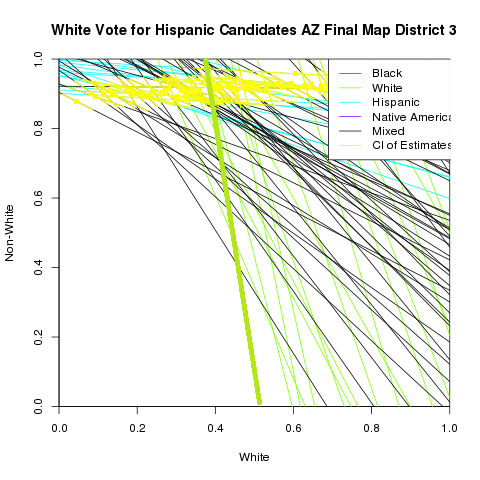
\includegraphics[scale=1]{figs/pl_whitevote_h_3_ld.png}
\caption{\label{tomog}This tomography plot displays the white vote for the Hispanic
  Candidate in 2010 Mine Inspector Election}
\end{center}
\end{figure}

For example, consider the bold green line in the plot. We know, based
on the observed data from that precinct (the percent voting and the
percent Hispanic), that the point in this plot (representing where the
White and non-White vote share is) for this precinct must be some
point on the line, but we do not know exactly where on the line this
point falls. For this line, we know that the fraction of Whites that
vote for the Hispanic candidate must fall somewhere between 0.42 (42
percent) and 0.52 (52 percent). We get these numbers by projecting the
line downwards to the horizontal axis. If instead we project the line
to the left (vertical) axis, we can see that, for this particular
precinct, the range of possible values for the percent of non-Whites
voting for the Hispanic candidate could be anywhere from 0\% to 100\%.
That estimate is better than the method of ecological regression,
which often gives answers outside that interval, but still we can see
that this precinct is informative with respect only to Whites, not
non-Whites. 

In this way, each line on a tomography plot captures exactly what we
do and do not know about the voting behavior in each precinct ---
without any uncertainty (assuming only that the data are measured
correctly). Our statistical method then uses all this available
information as well as the statistical information from ecological
regression. Lines that are relatively steep in this particular
tomography plot convey a lot of information about the percent of
Whites that vote for the Hispanic candidate.  Lines that are
relatively flat convey a great deal of information about the percent
of non-Whites voting for the Hispanic candidate.  Lines that cut off
the top right or bottom left corner of the plot are informative about
both quantities.

The tomography plots reflect what we know about the racial composition
of each precinct. If a precinct contains more than 65\% of a
particular racial group (which we use as an arbitrary cutoff for
graphical clarity), then the line on the tomography plot that
corresponds to that precinct is color coded to represent the majority
group (see the legend in the plot). If no groups comprise 65\% or more
of the precinct, then no color code is assigned.  

Finally, the tomography plots also reflect the results of the
ecological inference statistical estimation, that includes information
on patterns across precincts. The point estimate (i.e., the exact
point on the line that we estimate as the vote share for each group)
as well as the confidence intervals are colored yellow.  Taken
together, these describe the overall estimate of how racial groups
voted in the district as a whole. For example, in the tomography plot
for District 3 in Figure \ref{tomog}, the mass of yellow in the top left
part of the graph means that our estimates indicate that whites likely voted for the Hispanic candidate at a lower rate than did their
non-white counterparts in the district.  

As importantly, the tomography plots convey the \emph{overall
  uncertainty} in the available data, and how our statistical
estimator uses that information to produce an estimate.  In this
particular example, the prevalence of flat lines near the top and
steep lines near the left convey a great deal of information about
where and what we are uncertain about.  The statistical estimator
assumes that there is some relationship among all the precincts in a
district, and so in all likelihood there exists a cluster of points on
the plot somewhere such that when two lines cross or approach one
another, the true points on each are close to each other on their
respective lines.  

To appropriately and completely judge all sources of uncertainty in
ecological inferences requires examining a plot like this for each
numerical quantity to be estimated.  The uncertainty estimates here
are far more informative and information rich than sampling based
confidence intervals or standard errors, which assume the model is
true and only summarize fundamental and estimation uncertainty.  Our
appendix includes all such plots, calculated for all offices we
analyzed, for VAP and CVAP, and for each district.

\section{Results for the Legislative Plan}\label{s:res}

The benchmark legislative districts in the analysis are LDs 2, 13, 14, 15, 16, 23, 24, 25, 27, and 29. The proposed legislative districts in the analysis are LDs 2, 3, 4, 7, 19, 24, 26, 27, 29, and 30. 

\subsection{Racially Polarized Voting}

We now assess the degree of racially polarized voting in both the
benchmark and proposed districts.  We do this with detailed tables in
the appendix (and far more extensive ones on our web appendix), and a
graphic summary of all of this information.

%analysis of polarized voting

\begin{figure}[p!h]
\begin{center}
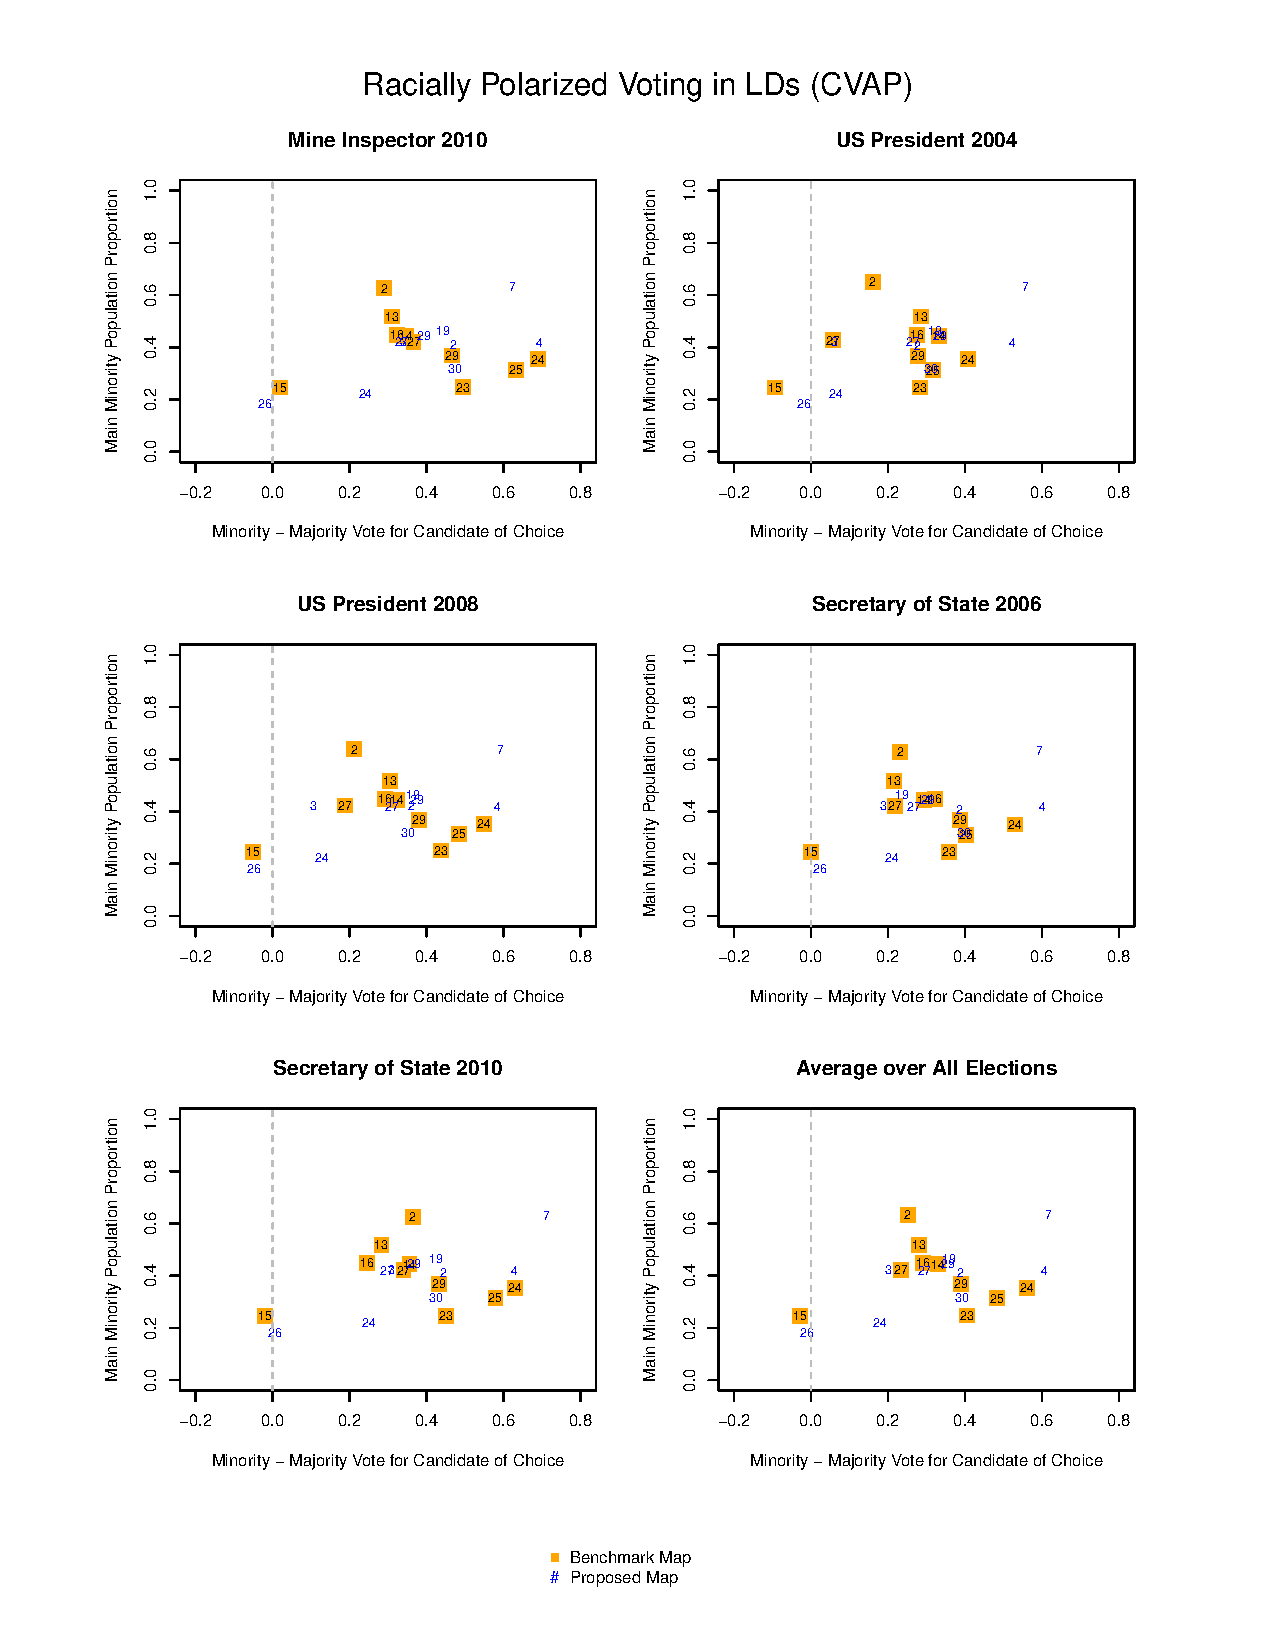
\includegraphics[scale=.8]{figs/cvap_ld_polarization.pdf}
\caption{\label{cvap_ld_polarization}CVAP Legislative Districts}
\end{center}
\end{figure}

We also offer here a summary of the vast array of results in a
convenient set of graphs.  First, Figure~\ref{cvap_ld_polarization}
displays the level of racially polarized voting across all races and
also provides an easy graphical means of comparing racial polarization
between the proposed and benchmark districts.

In each graph in this figure, the horizontal axis represents the main
minority vote minus the majority (white) vote for each
district.  The first five graphs repeat the same analysis with
different statewide races, and the bottom right graph summarizes the
five graphs by presenting an average.  The similarity across the five
graphs reflects the similarity in this aspect of voting patterns
across the different statewide offices.  In each of the graphs, the
districts located farther to the right exhibit higher levels of
racially polarized voting. The vertical axis tracks the share of the
main minority population in each district. The orange
squares represent the location of the benchmark districts while the
blue numbers represent the proposed districts.

As the figure illustrates, the majority of legislative districts in both the benchmark and proposed LDs exhibit racially polarized voting across all races. However, there are some notable exceptions. According to our estimates, proposed LD 26 exhibits little racial polarization in the voting patterns. In fact, for several elections we estimate that the majority group voted for the minority candidate at a higher rate than did the main minority group. Similarly, benchmark LD 15 exhibited very similar behavior in terms of a lack of racially polarized voting.

Several other districts also exhibited lower levels of racial polarization depending on the election. Proposed LDs 2 and 24 exhibited relatively lower levels of polarization in the US President 2004 and US President 2008 elections. Benchmark LD 27 exhibited a noticeably lower level of racial polarization for the US President 2004 election. Nonetheless, as the graph displaying the average results over all five elections demonstrates, all districts but benchmark LD 15 and proposed LD 26 exhibited a level of polarized voting of close to at least 20\%.

\subsection{Electability of Candidate of Choice}

Here we assess the electability of the candidate of choice in both the
benchmark and proposed districts.

%analysis of electability

Figure~\ref{cvap_ld} gives a graphical summary of our results; this
figure is particularly crucial because it helps provide answers to the
questions that are at the heart of whether the proposed districts are
retrogressive or not. In particular, for each election the figure
captures (1) the {\it estimated} level of support among the main
minority group in each legislative district candidate for the
candidate of choice; (2) the {\it observed} electability of the
candidate of choice in each legislative district; and, (3) the
degree to which the proposed districts represent improvement or
retrogression along dimensions 1 and 2.

Again, each graph in Figure~\ref{cvap_ld} performs an analysis based
on a different statewide office, with the average appearing in the
bottom right.  In each, the horizontal axis captures the estimated
(two-party) vote share for the candidate of choice among the main
minority population. The vertical axis represents the observed
(two-party) vote share for the candidate of choice among all voters in
the district.  When a district falls in the top right quadrant of a
graph it means that that (1) the main minority in the district prefers
the candidate of choice and (2) the district as a whole would have
elected the candidate of choice.

\begin{figure}[p!h]
\begin{center}
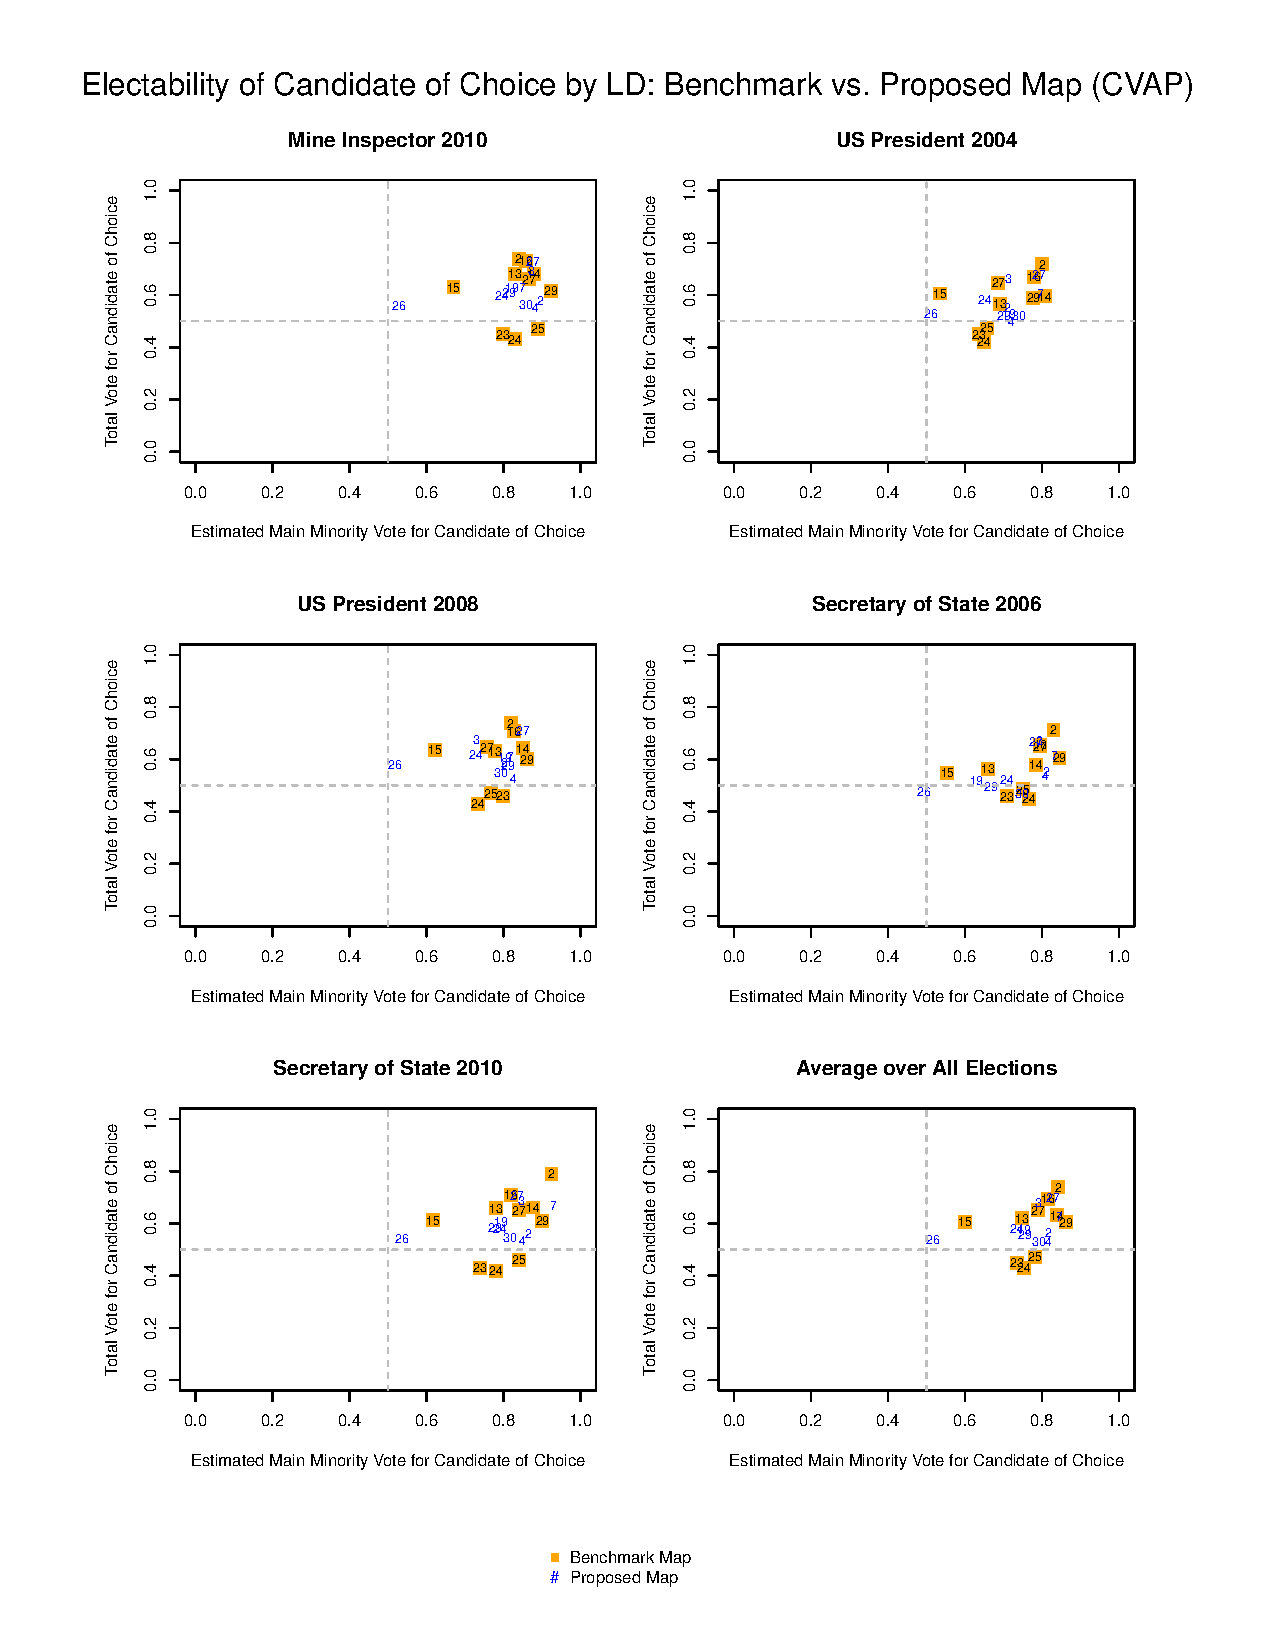
\includegraphics[scale=.8]{figs/cvap_ld.pdf}
\caption{\label{cvap_ld}CVAP Legislative Districts}
\end{center}
\end{figure}

For each graph in Figure~\ref{cvap_ld}, the horizontal axis displays the estimated two-party vote share for the candidate of choice among the main minority population. The vertical axis represents the observed two-party vote share for the candidate of choice in the district. Thus, when a district falls in the top right quadrant of a graph it means that that the main minority in the district prefers the candidate of choice and the district as a whole would have elected the candidate of choice. 

First, we examine the benchmark districts. Across all elections, we note that benchmark LDs 23, 24 and 25 demonstrate support for the candidate of choice among the main minority group; however, none of these districts are ever actually able to elect the candidate of choice. This is evident from the graphs because these three districts fall in the bottom right quadrant rather than the top right quadrant in each graph. Other than these three districts, the remaining benchmark LDs exhibit the ability to elect the candidate of choice. The only issue is that in benchmark LD 15 it is sometimes not clear if the expected candidate of choice is strongly preferred by the main minority group. For example, in the US President 2004 election, we estimate that Hispanics in LD 15 voted for the Democratic candidate at a rate of 53\%, which is by no means overwhelming support for the candidate of choice. 

Moving to an analysis of the proposed LDs, the most important thing to note is that no districts perform as consistently poorly in terms of ability to elect the candidate of choice as do benchmark LDs 23, 24, and 25. In fact, averaging across all elections it is clear that all proposed LDs fall in the upper right hand quadrant. Furthermore, all proposed LDs other than LD 26 demonstrate that there is clear main minority support for the candidate of choice in each election. Other than LD 26, the lowest estimated level of support for the candidate of choice among the main minority group is in LD 19, where Hispanic voters voted for the Democratic candidate for Secretary of State in 2006 at an estimated rate of 60\%. 

In terms of ability to elect the candidate of choice, the proposed LDs also outperform the benchmark LDs. On average, all districts vote for the candidate of choice at a rate that is substantially higher than in benchmark LDs 23, 24, or 25. Of the five elections we examined, only in the election for Secretary of State 2006 did the overall ability to elect the candidate of choice seem to be in question in more than one district. But even in this case the districts outperformed the benchmark LDs.

LD 26 is clearly the one proposed district for which both the support for the candidate of choice among the main minority group as well as the overall ability to elect comes into question. There are several factors at play in LD 26 worth keeping in mind. First, we have estimated that there is a low level of polarized voting between Hispanic and white voters in the district. Furthermore, because of the nature of the district, our estimates based on ecological inference are relatively uncertain in LD 26. Figure~\ref{tomog_26} helps illustrate the issue. It displays the tomography plot for the Hispanic vote for the Hispanic Democratic candidate in the 2010 Mine Inspector Election. The horizontal axis displays the vote share for this candidate among Hispanic voters. 

\begin{figure}[htb]
\begin{center}
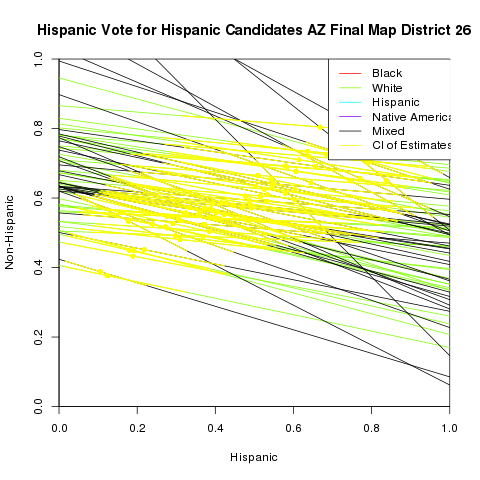
\includegraphics[scale=.75]{figs/pl_hispvote_h_26_smine.png}
\caption{\label{tomog_26}This tomography plot displays the Hispanic vote for the Hispanic Candidate in 2010 Mine Inspector Election}
\end{center}
\end{figure}

Because of the combination of voting patterns along with a relatively smaller Hispanic population (CVAP), there is a high degree of uncertainty in the estimates for this district. As the tomography plot illustrates, most of the lines are horizontal, which means there is very little concrete information that we can infer about how Hispanic voters are voting. In fact, without performing any inference we can only say that the bound on vote share for the Hispanic candidate among Hispanic voters is somewhere between 0 and 1. While this plot is just for the Mine Inspector election, the tomography plots for other elections in LD 26 are very similar. 

Based on the empirical evidence available, we conclude that LD 26 does not appear to exhibit polarized voting between whites and Hispanics; furthermore, the level of support among Hispanic voters for the expected candidate of choice (i.e., the candidate who is an ethnic minority or who appears to be the preferred choice of minority groups) is not clear. Importantly, this is not a problem with how the district has been drawn; rather, it is just a product of how people vote and where people live in the district. Despite these caveats, however, the minority candidate still wins in LD 26 in four of the five elections that we examine. The same cannot be said about three of the ten benchmark districts.

\subsection{Could Stronger Districts Have been Drawn?}

While the analysis in the previous section revealed that the proposed districts
demonstrate a greater ability to elect the candidate of choice than the benchmark districts, 
we still hope to learn whether even stronger districts could have been drawn.
The \emph{performance analysis} that we described above helps answer this question.

Figure~\ref{cvap_ld_performance_ratio} summarizes the results from
running the performance analysis for each district and election.
The full results are available in our web appendix. The horizontal
axis in the figure is the change in Hispanic population share required
to reach the 55\% threshold for the candidate of choice. If a district
is plotted to the left of the origin (i.e., left of the vertical
dashed line at zero), then initially the district vote totals for the
candidate of choice were greater than the 55\% threshold and so we
envision what would occur if we removed Hispanic voters from the
district. If the district is plotted to the right of the origin, then
initially the district vote totals for the candidate of choice were
less than the 55\% threshold and so we envision what would occur if we
added Hispanic voters to the district.

In some cases, even if we examine the counterfactual in which we have
changed the composition of the district as much as possible (for
example, constructing a district that contains 0\% or 100\% Hispanics)
it is still not possible to reach the target threshold. This would
occur for example in a district where the candidate of choice receives
fewer than 55\% of the vote, and even Hispanic voters in the
neighboring districts do not favor the candidate of choice. These cases 
are denoted in red in Figure~\ref{cvap_ld_performance_ratio}, and they suggest
that it would be difficult to strengthen these districts.

The vertical axis represents the ratio of vote share change to
population change. This is essentially a measure of ``bang for the
buck''. It tells us the relative amount that we had to alter the
composition of the district in order to gain an additional percentage
point in vote for the candidate of choice. Thus, a district that is
located relatively higher on the vertical axis is one for which
changes in the composition of the district result in relatively more
changes in voting patterns.

\begin{figure}[p!h]
\begin{center}
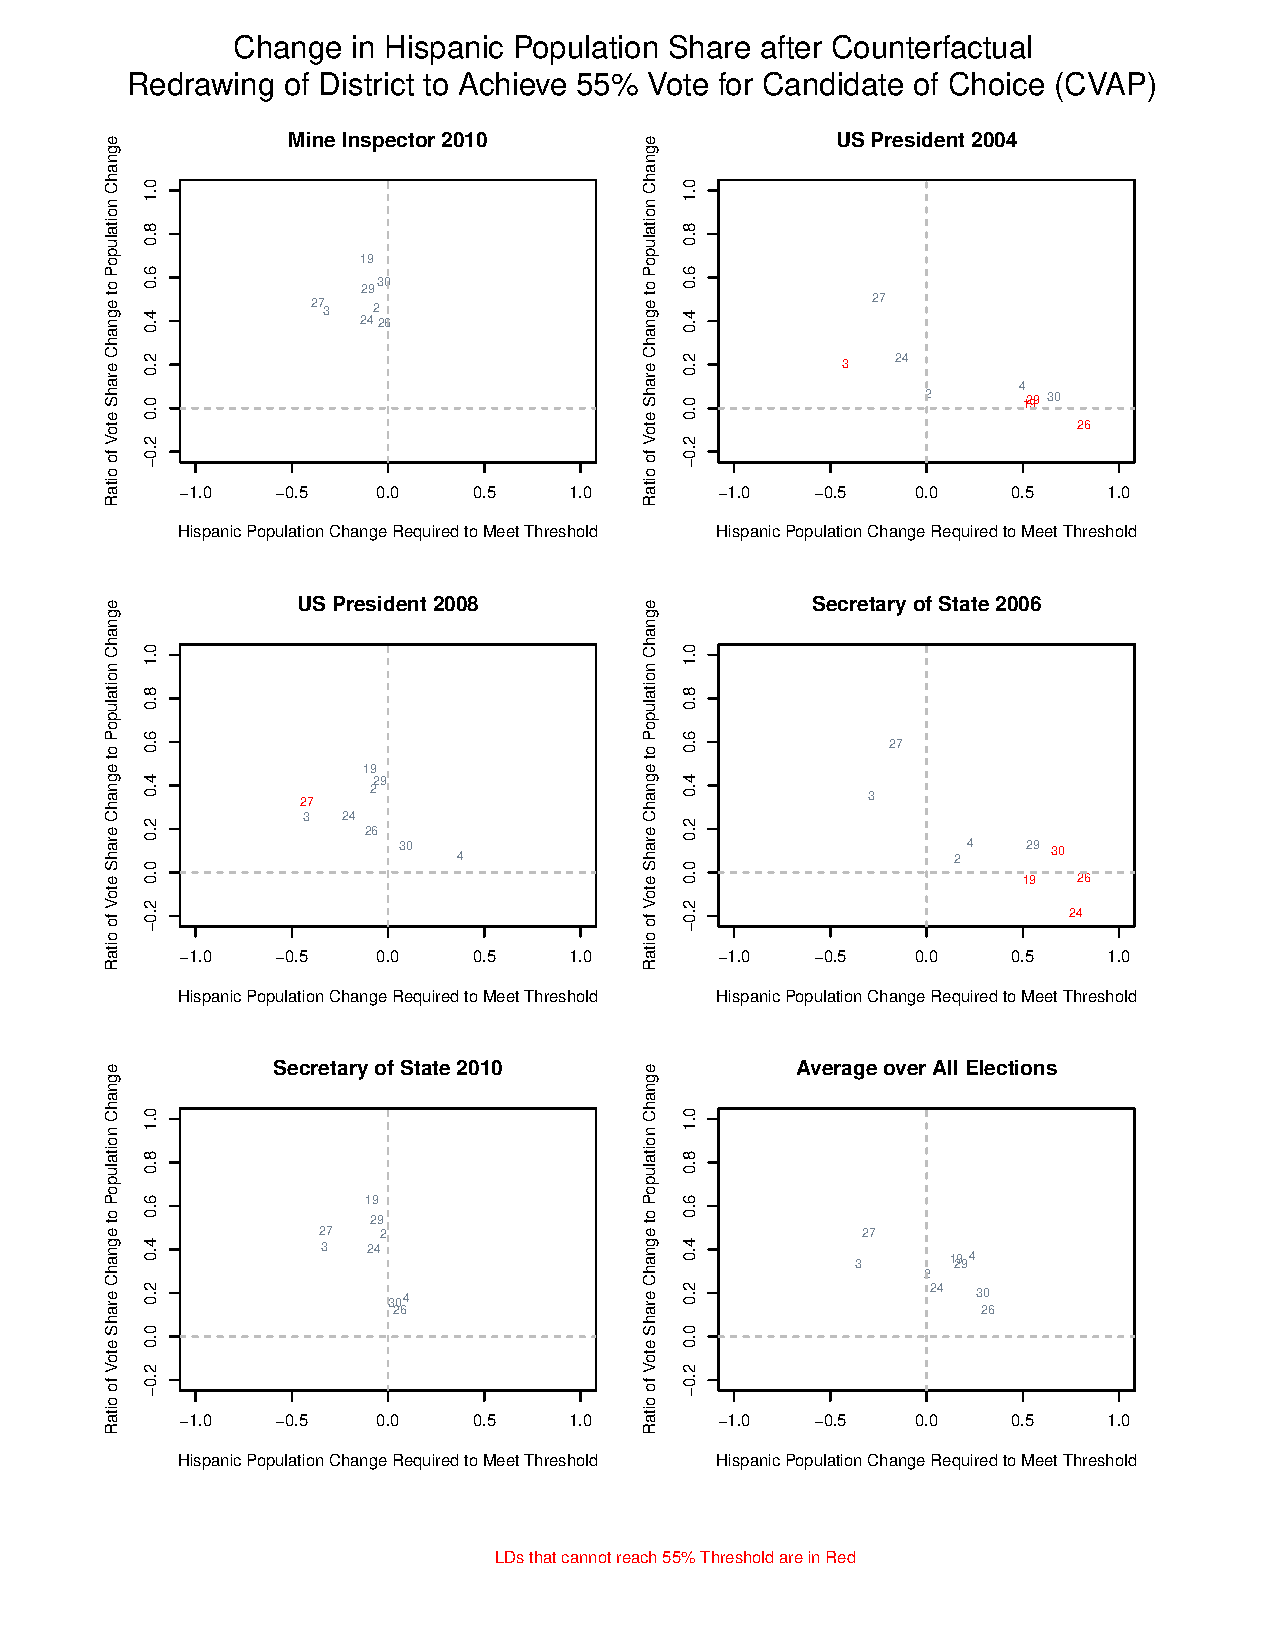
\includegraphics[scale=.8]{figs/cvap_ld_performance_ratio.pdf}
\caption{\label{cvap_ld_performance_ratio}CVAP Legislative Districts}
\end{center}
\end{figure}

Starting with the Mine Inspector 2010 graph in the upper left hand corner, we see that most districts were already above the 55\% threshold. The US President 2004 graph is more interesting; we estimate that for several districts -- LD 19, 26, and 29 -- it would not be possible to raise the overall vote share for the candidate of choice to 55\% by tweaking the district lines. The same is true of several districts when we examine the Secretary of State 2006 election. 

The graphs also provide useful information about how difficult it would be to strengthen any districts that appeared weaker in the previous analysis. These graphs suggest that altering the lines of LD 26 would likely not be an effective way to strengthen the district. In two of the five elections, we estimate that it would be impossible to strengthen LD 26 sufficiently to reach a 55\% threshold for the candidate of choice while drawing from adjacent non-VRA districts. In the remaining three elections, the efficiency of redrawing LD 26 appears relatively low. Specifically, we estimate that relatively large changes in the composition of the district would have to occur in order to sufficiently shore up support for the candidate of choice. This is perhaps best illustrated by the graph displaying the average result over all elections. In this graph, LD 26 has the lowest ratio of vote share change to population change required of any of the minority districts.

\clearpage
\appendix

\section{Appendix: CVAP-Based Ecological Inference Estimates}
\subsection{Proposed Map}

% latex table generated in R 2.13.1 by xtable 1.6-0 package
% Thu Jan 26 11:22:22 2012
\begin{table}[htb]
\begin{center}
\caption{Mine Inspector 2010 LD 2 (Proposed)}
\label{smine_cvap_ld_2}
\begin{tabular}{lccccc}
  \hline
Racial Group & Turnout & D Vote & R Vote & S Vote & Total CVAP \\ 
  \hline
White & 0.51 & 0.43 & 0.57 & 0.00 & 0.49 \\ 
  Hispanic & 0.28 & 0.89 & 0.10 & 0.00 & 0.41 \\ 
  Native American & 0.35 & 0.76 & 0.23 & 0.01 & 0.02 \\ 
  Black & 0.18 & 0.52 & 0.47 & 0.01 & 0.04 \\ 
  Other & 0.24 & 0.56 & 0.43 & 0.01 & 0.04 \\ 
  Total Pop & 0.39 & 0.58 & 0.42 & 0.00 &  \\ 
   \hline
\end{tabular}
\end{center}
\end{table}

% latex table generated in R 2.13.1 by xtable 1.6-0 package
% Thu Jan 26 11:22:22 2012
\begin{table}[htb]
\begin{center}
\caption{Mine Inspector 2010 LD 3 (Proposed)}
\label{smine_cvap_ld_3}
\begin{tabular}{lccccc}
  \hline
Racial Group & Turnout & D Vote & R Vote & S Vote & Total CVAP \\ 
  \hline
White & 0.33 & 0.53 & 0.47 & 0.00 & 0.45 \\ 
  Hispanic & 0.33 & 0.87 & 0.13 & 0.00 & 0.42 \\ 
  Native American & 0.21 & 0.74 & 0.25 & 0.01 & 0.04 \\ 
  Black & 0.30 & 0.64 & 0.35 & 0.01 & 0.03 \\ 
  Other & 0.45 & 0.65 & 0.34 & 0.00 & 0.05 \\ 
  Total Pop & 0.33 & 0.69 & 0.31 & 0.00 &  \\ 
   \hline
\end{tabular}
\end{center}
\end{table}

% latex table generated in R 2.13.1 by xtable 1.6-0 package
% Thu Jan 26 11:22:22 2012
\begin{table}[htb]
\begin{center}
\caption{Mine Inspector 2010 LD 4 (Proposed)}
\label{smine_cvap_ld_4}
\begin{tabular}{lccccc}
  \hline
Racial Group & Turnout & D Vote & R Vote & S Vote & Total CVAP \\ 
  \hline
White & 0.32 & 0.19 & 0.81 & 0.00 & 0.42 \\ 
  Hispanic & 0.28 & 0.88 & 0.12 & 0.00 & 0.42 \\ 
  Native American & 0.22 & 0.92 & 0.08 & 0.01 & 0.07 \\ 
  Black & 0.38 & 0.64 & 0.35 & 0.01 & 0.04 \\ 
  Other & 0.42 & 0.75 & 0.25 & 0.01 & 0.05 \\ 
  Total Pop & 0.30 & 0.55 & 0.45 & 0.00 &  \\ 
   \hline
\end{tabular}
\end{center}
\end{table}

% latex table generated in R 2.13.1 by xtable 1.6-0 package
% Thu Jan 26 11:22:22 2012
\begin{table}[htb]
\begin{center}
\caption{Mine Inspector 2010 LD 7 (Proposed)}
\label{smine_cvap_ld_7}
\begin{tabular}{lccccc}
  \hline
Racial Group & Turnout & D Vote & R Vote & S Vote & Total CVAP \\ 
  \hline
White & 0.44 & 0.23 & 0.77 & 0.00 & 0.28 \\ 
  Hispanic & 0.25 & 0.55 & 0.45 & 0.01 & 0.05 \\ 
  Native American & 0.34 & 0.85 & 0.15 & 0.00 & 0.63 \\ 
  Black & 0.41 & 0.56 & 0.42 & 0.02 & 0.01 \\ 
  Other & 0.28 & 0.80 & 0.19 & 0.01 & 0.04 \\ 
  Total Pop & 0.36 & 0.63 & 0.37 & 0.00 &  \\ 
   \hline
\end{tabular}
\end{center}
\end{table}

%% latex table generated in R 2.13.1 by xtable 1.6-0 package
% Thu Jan 26 11:22:22 2012
\begin{table}[htb]
\begin{center}
\caption{Mine Inspector 2010 LD 8 (Proposed)}
\label{smine_cvap_ld_8}
\begin{tabular}{lccccc}
  \hline
Racial Group & Turnout & D Vote & R Vote & S Vote & Total CVAP \\ 
  \hline
White & 0.42 & 0.38 & 0.62 & 0.00 & 0.53 \\ 
  Hispanic & 0.18 & 0.83 & 0.17 & 0.00 & 0.30 \\ 
  Native American & 0.15 & 0.75 & 0.24 & 0.01 & 0.07 \\ 
  Black & 0.22 & 0.42 & 0.57 & 0.01 & 0.04 \\ 
  Other & 0.21 & 0.51 & 0.49 & 0.01 & 0.06 \\ 
  Total Pop & 0.31 & 0.48 & 0.52 & 0.00 &  \\ 
   \hline
\end{tabular}
\end{center}
\end{table}

% latex table generated in R 2.13.1 by xtable 1.6-0 package
% Thu Jan 26 11:22:22 2012
\begin{table}[htb]
\begin{center}
\caption{Mine Inspector 2010 LD 19 (Proposed)}
\label{smine_cvap_ld_19}
\begin{tabular}{lccccc}
  \hline
Racial Group & Turnout & D Vote & R Vote & S Vote & Total CVAP \\ 
  \hline
White & 0.22 & 0.38 & 0.62 & 0.00 & 0.38 \\ 
  Hispanic & 0.20 & 0.82 & 0.18 & 0.00 & 0.47 \\ 
  Native American & 0.20 & 0.47 & 0.50 & 0.04 & 0.02 \\ 
  Black & 0.45 & 0.66 & 0.33 & 0.00 & 0.09 \\ 
  Other & 0.48 & 0.67 & 0.33 & 0.01 & 0.05 \\ 
  Total Pop & 0.24 & 0.63 & 0.37 & 0.00 &  \\ 
   \hline
\end{tabular}
\end{center}
\end{table}

% latex table generated in R 2.13.1 by xtable 1.6-0 package
% Thu Jan 26 11:22:22 2012
\begin{table}[htb]
\begin{center}
\caption{Mine Inspector 2010 LD 24 (Proposed)}
\label{smine_cvap_ld_24}
\begin{tabular}{lccccc}
  \hline
Racial Group & Turnout & D Vote & R Vote & S Vote & Total CVAP \\ 
  \hline
White & 0.35 & 0.55 & 0.45 & 0.00 & 0.64 \\ 
  Hispanic & 0.14 & 0.79 & 0.20 & 0.01 & 0.22 \\ 
  Native American & 0.22 & 0.59 & 0.39 & 0.02 & 0.04 \\ 
  Black & 0.33 & 0.68 & 0.31 & 0.01 & 0.05 \\ 
  Other & 0.46 & 0.68 & 0.31 & 0.01 & 0.05 \\ 
  Total Pop & 0.30 & 0.60 & 0.40 & 0.00 &  \\ 
   \hline
\end{tabular}
\end{center}
\end{table}

% latex table generated in R 2.13.1 by xtable 1.6-0 package
% Thu Jan 26 11:22:22 2012
\begin{table}[htb]
\begin{center}
\caption{Mine Inspector 2010 LD 26 (Proposed)}
\label{smine_cvap_ld_26}
\begin{tabular}{lccccc}
  \hline
Racial Group & Turnout & D Vote & R Vote & S Vote & Total CVAP \\ 
  \hline
White & 0.27 & 0.55 & 0.45 & 0.00 & 0.65 \\ 
  Hispanic & 0.15 & 0.52 & 0.47 & 0.01 & 0.18 \\ 
  Native American & 0.31 & 0.65 & 0.34 & 0.01 & 0.06 \\ 
  Black & 0.29 & 0.59 & 0.40 & 0.01 & 0.05 \\ 
  Other & 0.29 & 0.58 & 0.40 & 0.01 & 0.06 \\ 
  Total Pop & 0.25 & 0.56 & 0.44 & 0.00 &  \\ 
   \hline
\end{tabular}
\end{center}
\end{table}

% latex table generated in R 2.13.1 by xtable 1.6-0 package
% Thu Jan 26 11:22:22 2012
\begin{table}[htb]
\begin{center}
\caption{Mine Inspector 2010 LD 27 (Proposed)}
\label{smine_cvap_ld_27}
\begin{tabular}{lccccc}
  \hline
Racial Group & Turnout & D Vote & R Vote & S Vote & Total CVAP \\ 
  \hline
White & 0.30 & 0.54 & 0.46 & 0.00 & 0.30 \\ 
  Hispanic & 0.21 & 0.87 & 0.12 & 0.00 & 0.42 \\ 
  Native American & 0.15 & 0.80 & 0.18 & 0.02 & 0.05 \\ 
  Black & 0.33 & 0.79 & 0.21 & 0.00 & 0.18 \\ 
  Other & 0.40 & 0.68 & 0.31 & 0.01 & 0.06 \\ 
  Total Pop & 0.26 & 0.73 & 0.27 & 0.00 &  \\ 
   \hline
\end{tabular}
\end{center}
\end{table}

% latex table generated in R 2.13.1 by xtable 1.6-0 package
% Thu Jan 26 11:22:22 2012
\begin{table}[htb]
\begin{center}
\caption{Mine Inspector 2010 LD 29 (Proposed)}
\label{smine_cvap_ld_29}
\begin{tabular}{lccccc}
  \hline
Racial Group & Turnout & D Vote & R Vote & S Vote & Total CVAP \\ 
  \hline
White & 0.26 & 0.42 & 0.58 & 0.00 & 0.41 \\ 
  Hispanic & 0.19 & 0.81 & 0.18 & 0.00 & 0.45 \\ 
  Native American & 0.60 & 0.55 & 0.43 & 0.02 & 0.01 \\ 
  Black & 0.42 & 0.65 & 0.34 & 0.01 & 0.08 \\ 
  Other & 0.44 & 0.65 & 0.34 & 0.01 & 0.05 \\ 
  Total Pop & 0.26 & 0.61 & 0.39 & 0.00 &  \\ 
   \hline
\end{tabular}
\end{center}
\end{table}

% latex table generated in R 2.13.1 by xtable 1.6-0 package
% Thu Jan 26 11:22:22 2012
\begin{table}[htb]
\begin{center}
\caption{Mine Inspector 2010 LD 30 (Proposed)}
\label{smine_cvap_ld_30}
\begin{tabular}{lccccc}
  \hline
Racial Group & Turnout & D Vote & R Vote & S Vote & Total CVAP \\ 
  \hline
White & 0.24 & 0.38 & 0.61 & 0.00 & 0.52 \\ 
  Hispanic & 0.21 & 0.86 & 0.14 & 0.00 & 0.32 \\ 
  Native American & 0.23 & 0.67 & 0.31 & 0.02 & 0.04 \\ 
  Black & 0.25 & 0.46 & 0.53 & 0.01 & 0.06 \\ 
  Other & 0.38 & 0.69 & 0.31 & 0.01 & 0.07 \\ 
  Total Pop & 0.24 & 0.56 & 0.44 & 0.00 &  \\ 
   \hline
\end{tabular}
\end{center}
\end{table}

\clearpage
% latex table generated in R 2.13.1 by xtable 1.6-0 package
% Thu Jan 26 11:22:22 2012
\begin{table}[htb]
\begin{center}
\caption{US President 2004 LD 2 (Proposed)}
\label{pres04_cvap_ld_2}
\begin{tabular}{lccccc}
  \hline
Racial Group & Turnout & D Vote & R Vote & S Vote & Total CVAP \\ 
  \hline
White & 0.46 & 0.43 & 0.56 & 0.00 & 0.50 \\ 
  Hispanic & 0.38 & 0.71 & 0.29 & 0.01 & 0.41 \\ 
  Native American & 0.58 & 0.71 & 0.27 & 0.02 & 0.02 \\ 
  Black & 0.18 & 0.51 & 0.44 & 0.05 & 0.04 \\ 
  Other & 0.46 & 0.55 & 0.42 & 0.03 & 0.04 \\ 
  Total Pop & 0.42 & 0.55 & 0.44 & 0.01 &  \\ 
   \hline
\end{tabular}
\end{center}
\end{table}

% latex table generated in R 2.13.1 by xtable 1.6-0 package
% Thu Jan 26 11:22:23 2012
\begin{table}[htb]
\begin{center}
\caption{US President 2004 LD 3 (Proposed)}
\label{pres04_cvap_ld_3}
\begin{tabular}{lccccc}
  \hline
Racial Group & Turnout & D Vote & R Vote & S Vote & Total CVAP \\ 
  \hline
White & 0.54 & 0.65 & 0.35 & 0.00 & 0.45 \\ 
  Hispanic & 0.42 & 0.71 & 0.29 & 0.00 & 0.42 \\ 
  Native American & 0.15 & 0.55 & 0.38 & 0.07 & 0.04 \\ 
  Black & 0.46 & 0.55 & 0.42 & 0.03 & 0.03 \\ 
  Other & 0.35 & 0.43 & 0.52 & 0.05 & 0.05 \\ 
  Total Pop & 0.46 & 0.66 & 0.33 & 0.01 &  \\ 
   \hline
\end{tabular}
\end{center}
\end{table}

% latex table generated in R 2.13.1 by xtable 1.6-0 package
% Thu Jan 26 11:22:23 2012
\begin{table}[htb]
\begin{center}
\caption{US President 2004 LD 4 (Proposed)}
\label{pres04_cvap_ld_4}
\begin{tabular}{lccccc}
  \hline
Racial Group & Turnout & D Vote & R Vote & S Vote & Total CVAP \\ 
  \hline
White & 0.33 & 0.20 & 0.80 & 0.00 & 0.42 \\ 
  Hispanic & 0.39 & 0.72 & 0.28 & 0.00 & 0.42 \\ 
  Native American & 0.53 & 0.66 & 0.33 & 0.01 & 0.07 \\ 
  Black & 0.30 & 0.40 & 0.57 & 0.03 & 0.04 \\ 
  Other & 0.26 & 0.60 & 0.36 & 0.04 & 0.05 \\ 
  Total Pop & 0.36 & 0.50 & 0.50 & 0.01 &  \\ 
   \hline
\end{tabular}
\end{center}
\end{table}

% latex table generated in R 2.13.1 by xtable 1.6-0 package
% Thu Jan 26 11:22:23 2012
\begin{table}[htb]
\begin{center}
\caption{US President 2004 LD 7 (Proposed)}
\label{pres04_cvap_ld_7}
\begin{tabular}{lccccc}
  \hline
Racial Group & Turnout & D Vote & R Vote & S Vote & Total CVAP \\ 
  \hline
White & 0.48 & 0.24 & 0.76 & 0.01 & 0.28 \\ 
  Hispanic & 0.17 & 0.57 & 0.37 & 0.07 & 0.05 \\ 
  Native American & 0.41 & 0.79 & 0.20 & 0.00 & 0.63 \\ 
  Black & 0.31 & 0.42 & 0.48 & 0.10 & 0.01 \\ 
  Other & 0.23 & 0.46 & 0.48 & 0.06 & 0.04 \\ 
  Total Pop & 0.41 & 0.60 & 0.39 & 0.01 &  \\ 
   \hline
\end{tabular}
\end{center}
\end{table}

%% latex table generated in R 2.13.1 by xtable 1.6-0 package
% Thu Jan 26 11:22:23 2012
\begin{table}[htb]
\begin{center}
\caption{US President 2004 LD 8 (Proposed)}
\label{pres04_cvap_ld_8}
\begin{tabular}{lccccc}
  \hline
Racial Group & Turnout & D Vote & R Vote & S Vote & Total CVAP \\ 
  \hline
White & 0.32 & 0.31 & 0.69 & 0.00 & 0.53 \\ 
  Hispanic & 0.36 & 0.70 & 0.30 & 0.01 & 0.30 \\ 
  Native American & 0.14 & 0.46 & 0.51 & 0.03 & 0.07 \\ 
  Black & 0.42 & 0.35 & 0.64 & 0.02 & 0.04 \\ 
  Other & 0.34 & 0.47 & 0.50 & 0.03 & 0.05 \\ 
  Total Pop & 0.32 & 0.45 & 0.54 & 0.01 &  \\ 
   \hline
\end{tabular}
\end{center}
\end{table}

% latex table generated in R 2.13.1 by xtable 1.6-0 package
% Thu Jan 26 11:22:23 2012
\begin{table}[htb]
\begin{center}
\caption{US President 2004 LD 19 (Proposed)}
\label{pres04_cvap_ld_19}
\begin{tabular}{lccccc}
  \hline
Racial Group & Turnout & D Vote & R Vote & S Vote & Total CVAP \\ 
  \hline
White & 0.30 & 0.39 & 0.60 & 0.00 & 0.38 \\ 
  Hispanic & 0.19 & 0.71 & 0.28 & 0.01 & 0.47 \\ 
  Native American & 0.53 & 0.53 & 0.43 & 0.04 & 0.02 \\ 
  Black & 0.70 & 0.50 & 0.49 & 0.01 & 0.09 \\ 
  Other & 0.51 & 0.51 & 0.48 & 0.01 & 0.05 \\ 
  Total Pop & 0.30 & 0.52 & 0.47 & 0.01 &  \\ 
   \hline
\end{tabular}
\end{center}
\end{table}

% latex table generated in R 2.13.1 by xtable 1.6-0 package
% Thu Jan 26 11:22:23 2012
\begin{table}[htb]
\begin{center}
\caption{US President 2004 LD 24 (Proposed)}
\label{pres04_cvap_ld_24}
\begin{tabular}{lccccc}
  \hline
Racial Group & Turnout & D Vote & R Vote & S Vote & Total CVAP \\ 
  \hline
White & 0.56 & 0.58 & 0.41 & 0.00 & 0.64 \\ 
  Hispanic & 0.22 & 0.64 & 0.34 & 0.02 & 0.22 \\ 
  Native American & 0.28 & 0.47 & 0.47 & 0.06 & 0.04 \\ 
  Black & 0.38 & 0.54 & 0.42 & 0.04 & 0.05 \\ 
  Other & 0.46 & 0.44 & 0.52 & 0.04 & 0.05 \\ 
  Total Pop & 0.46 & 0.58 & 0.41 & 0.01 &  \\ 
   \hline
\end{tabular}
\end{center}
\end{table}

% latex table generated in R 2.13.1 by xtable 1.6-0 package
% Thu Jan 26 11:22:23 2012
\begin{table}[htb]
\begin{center}
\caption{US President 2004 LD 26 (Proposed)}
\label{pres04_cvap_ld_26}
\begin{tabular}{lccccc}
  \hline
Racial Group & Turnout & D Vote & R Vote & S Vote & Total CVAP \\ 
  \hline
White & 0.48 & 0.53 & 0.47 & 0.00 & 0.65 \\ 
  Hispanic & 0.26 & 0.50 & 0.48 & 0.02 & 0.18 \\ 
  Native American & 0.39 & 0.51 & 0.46 & 0.03 & 0.06 \\ 
  Black & 0.40 & 0.57 & 0.39 & 0.04 & 0.05 \\ 
  Other & 0.29 & 0.51 & 0.44 & 0.05 & 0.06 \\ 
  Total Pop & 0.42 & 0.53 & 0.47 & 0.01 &  \\ 
   \hline
\end{tabular}
\end{center}
\end{table}

% latex table generated in R 2.13.1 by xtable 1.6-0 package
% Thu Jan 26 11:22:23 2012
\begin{table}[htb]
\begin{center}
\caption{US President 2004 LD 27 (Proposed)}
\label{pres04_cvap_ld_27}
\begin{tabular}{lccccc}
  \hline
Racial Group & Turnout & D Vote & R Vote & S Vote & Total CVAP \\ 
  \hline
White & 0.24 & 0.52 & 0.47 & 0.01 & 0.30 \\ 
  Hispanic & 0.35 & 0.79 & 0.21 & 0.00 & 0.42 \\ 
  Native American & 0.17 & 0.55 & 0.42 & 0.04 & 0.05 \\ 
  Black & 0.32 & 0.62 & 0.38 & 0.01 & 0.18 \\ 
  Other & 0.22 & 0.49 & 0.48 & 0.03 & 0.06 \\ 
  Total Pop & 0.30 & 0.67 & 0.32 & 0.01 &  \\ 
   \hline
\end{tabular}
\end{center}
\end{table}

% latex table generated in R 2.13.1 by xtable 1.6-0 package
% Thu Jan 26 11:22:23 2012
\begin{table}[htb]
\begin{center}
\caption{US President 2004 LD 29 (Proposed)}
\label{pres04_cvap_ld_29}
\begin{tabular}{lccccc}
  \hline
Racial Group & Turnout & D Vote & R Vote & S Vote & Total CVAP \\ 
  \hline
White & 0.38 & 0.37 & 0.63 & 0.00 & 0.41 \\ 
  Hispanic & 0.30 & 0.70 & 0.30 & 0.01 & 0.45 \\ 
  Native American & 0.48 & 0.49 & 0.46 & 0.05 & 0.01 \\ 
  Black & 0.33 & 0.48 & 0.49 & 0.03 & 0.08 \\ 
  Other & 0.45 & 0.49 & 0.49 & 0.02 & 0.05 \\ 
  Total Pop & 0.34 & 0.52 & 0.48 & 0.01 &  \\ 
   \hline
\end{tabular}
\end{center}
\end{table}

% latex table generated in R 2.13.1 by xtable 1.6-0 package
% Thu Jan 26 11:22:23 2012
\begin{table}[htb]
\begin{center}
\caption{US President 2004 LD 30 (Proposed)}
\label{pres04_cvap_ld_30}
\begin{tabular}{lccccc}
  \hline
Racial Group & Turnout & D Vote & R Vote & S Vote & Total CVAP \\ 
  \hline
White & 0.40 & 0.43 & 0.57 & 0.00 & 0.52 \\ 
  Hispanic & 0.28 & 0.73 & 0.26 & 0.01 & 0.32 \\ 
  Native American & 0.39 & 0.55 & 0.42 & 0.03 & 0.04 \\ 
  Black & 0.30 & 0.46 & 0.51 & 0.03 & 0.06 \\ 
  Other & 0.29 & 0.49 & 0.47 & 0.04 & 0.07 \\ 
  Total Pop & 0.35 & 0.52 & 0.47 & 0.01 &  \\ 
   \hline
\end{tabular}
\end{center}
\end{table}

\clearpage
% latex table generated in R 2.13.1 by xtable 1.6-0 package
% Thu Jan 26 11:22:23 2012
\begin{table}[htb]
\begin{center}
\caption{US President 2008 LD 2 (Proposed)}
\label{pres08_cvap_ld_2}
\begin{tabular}{lccccc}
  \hline
Racial Group & Turnout & D Vote & R Vote & S Vote & Total CVAP \\ 
  \hline
White & 0.55 & 0.44 & 0.55 & 0.01 & 0.48 \\ 
  Hispanic & 0.41 & 0.80 & 0.20 & 0.01 & 0.42 \\ 
  Native American & 0.48 & 0.67 & 0.27 & 0.05 & 0.02 \\ 
  Black & 0.32 & 0.54 & 0.41 & 0.05 & 0.04 \\ 
  Other & 0.44 & 0.52 & 0.43 & 0.05 & 0.04 \\ 
  Total Pop & 0.48 & 0.58 & 0.41 & 0.01 &  \\ 
   \hline
\end{tabular}
\end{center}
\end{table}

% latex table generated in R 2.13.1 by xtable 1.6-0 package
% Thu Jan 26 11:22:23 2012
\begin{table}[htb]
\begin{center}
\caption{US President 2008 LD 3 (Proposed)}
\label{pres08_cvap_ld_3}
\begin{tabular}{lccccc}
  \hline
Racial Group & Turnout & D Vote & R Vote & S Vote & Total CVAP \\ 
  \hline
White & 0.48 & 0.62 & 0.37 & 0.01 & 0.45 \\ 
  Hispanic & 0.41 & 0.72 & 0.27 & 0.01 & 0.42 \\ 
  Native American & 0.27 & 0.70 & 0.22 & 0.07 & 0.04 \\ 
  Black & 0.41 & 0.59 & 0.35 & 0.06 & 0.03 \\ 
  Other & 0.66 & 0.68 & 0.28 & 0.04 & 0.05 \\ 
  Total Pop & 0.45 & 0.67 & 0.32 & 0.01 &  \\ 
   \hline
\end{tabular}
\end{center}
\end{table}

% latex table generated in R 2.13.1 by xtable 1.6-0 package
% Thu Jan 26 11:22:23 2012
\begin{table}[htb]
\begin{center}
\caption{US President 2008 LD 4 (Proposed)}
\label{pres08_cvap_ld_4}
\begin{tabular}{lccccc}
  \hline
Racial Group & Turnout & D Vote & R Vote & S Vote & Total CVAP \\ 
  \hline
White & 0.47 & 0.24 & 0.75 & 0.01 & 0.42 \\ 
  Hispanic & 0.37 & 0.82 & 0.17 & 0.01 & 0.42 \\ 
  Native American & 0.36 & 0.78 & 0.21 & 0.01 & 0.07 \\ 
  Black & 0.52 & 0.54 & 0.41 & 0.05 & 0.04 \\ 
  Other & 0.54 & 0.62 & 0.33 & 0.05 & 0.05 \\ 
  Total Pop & 0.43 & 0.52 & 0.47 & 0.01 &  \\ 
   \hline
\end{tabular}
\end{center}
\end{table}

% latex table generated in R 2.13.1 by xtable 1.6-0 package
% Thu Jan 26 11:22:23 2012
\begin{table}[htb]
\begin{center}
\caption{US President 2008 LD 7 (Proposed)}
\label{pres08_cvap_ld_7}
\begin{tabular}{lccccc}
  \hline
Racial Group & Turnout & D Vote & R Vote & S Vote & Total CVAP \\ 
  \hline
White & 0.54 & 0.22 & 0.77 & 0.01 & 0.27 \\ 
  Hispanic & 0.31 & 0.42 & 0.53 & 0.05 & 0.05 \\ 
  Native American & 0.42 & 0.81 & 0.18 & 0.01 & 0.64 \\ 
  Black & 0.54 & 0.47 & 0.44 & 0.09 & 0.01 \\ 
  Other & 0.50 & 0.72 & 0.21 & 0.07 & 0.04 \\ 
  Total Pop & 0.45 & 0.60 & 0.38 & 0.01 &  \\ 
   \hline
\end{tabular}
\end{center}
\end{table}

%% latex table generated in R 2.13.1 by xtable 1.6-0 package
% Thu Jan 26 11:22:23 2012
\begin{table}[htb]
\begin{center}
\caption{US President 2008 LD 8 (Proposed)}
\label{pres08_cvap_ld_8}
\begin{tabular}{lccccc}
  \hline
Racial Group & Turnout & D Vote & R Vote & S Vote & Total CVAP \\ 
  \hline
White & 0.53 & 0.36 & 0.64 & 0.01 & 0.52 \\ 
  Hispanic & 0.27 & 0.71 & 0.27 & 0.02 & 0.31 \\ 
  Native American & 0.27 & 0.58 & 0.39 & 0.02 & 0.08 \\ 
  Black & 0.32 & 0.40 & 0.55 & 0.06 & 0.04 \\ 
  Other & 0.29 & 0.42 & 0.50 & 0.08 & 0.06 \\ 
  Total Pop & 0.40 & 0.44 & 0.54 & 0.01 &  \\ 
   \hline
\end{tabular}
\end{center}
\end{table}

% latex table generated in R 2.13.1 by xtable 1.6-0 package
% Thu Jan 26 11:22:23 2012
\begin{table}[htb]
\begin{center}
\caption{US President 2008 LD 19 (Proposed)}
\label{pres08_cvap_ld_19}
\begin{tabular}{lccccc}
  \hline
Racial Group & Turnout & D Vote & R Vote & S Vote & Total CVAP \\ 
  \hline
White & 0.40 & 0.43 & 0.56 & 0.01 & 0.38 \\ 
  Hispanic & 0.29 & 0.80 & 0.20 & 0.01 & 0.46 \\ 
  Native American & 0.40 & 0.57 & 0.34 & 0.09 & 0.02 \\ 
  Black & 0.54 & 0.60 & 0.38 & 0.03 & 0.09 \\ 
  Other & 0.59 & 0.52 & 0.45 & 0.04 & 0.05 \\ 
  Total Pop & 0.37 & 0.60 & 0.39 & 0.01 &  \\ 
   \hline
\end{tabular}
\end{center}
\end{table}

% latex table generated in R 2.13.1 by xtable 1.6-0 package
% Thu Jan 26 11:22:23 2012
\begin{table}[htb]
\begin{center}
\caption{US President 2008 LD 24 (Proposed)}
\label{pres08_cvap_ld_24}
\begin{tabular}{lccccc}
  \hline
Racial Group & Turnout & D Vote & R Vote & S Vote & Total CVAP \\ 
  \hline
White & 0.55 & 0.60 & 0.40 & 0.01 & 0.64 \\ 
  Hispanic & 0.21 & 0.70 & 0.26 & 0.05 & 0.22 \\ 
  Native American & 0.35 & 0.53 & 0.39 & 0.08 & 0.04 \\ 
  Black & 0.47 & 0.65 & 0.28 & 0.07 & 0.05 \\ 
  Other & 0.55 & 0.51 & 0.39 & 0.09 & 0.05 \\ 
  Total Pop & 0.46 & 0.60 & 0.38 & 0.02 &  \\ 
   \hline
\end{tabular}
\end{center}
\end{table}

% latex table generated in R 2.13.1 by xtable 1.6-0 package
% Thu Jan 26 11:22:23 2012
\begin{table}[htb]
\begin{center}
\caption{US President 2008 LD 26 (Proposed)}
\label{pres08_cvap_ld_26}
\begin{tabular}{lccccc}
  \hline
Racial Group & Turnout & D Vote & R Vote & S Vote & Total CVAP \\ 
  \hline
White & 0.45 & 0.56 & 0.43 & 0.01 & 0.65 \\ 
  Hispanic & 0.20 & 0.48 & 0.45 & 0.07 & 0.18 \\ 
  Native American & 0.52 & 0.61 & 0.34 & 0.05 & 0.06 \\ 
  Black & 0.48 & 0.59 & 0.36 & 0.05 & 0.05 \\ 
  Other & 0.51 & 0.65 & 0.27 & 0.08 & 0.06 \\ 
  Total Pop & 0.41 & 0.57 & 0.41 & 0.02 &  \\ 
   \hline
\end{tabular}
\end{center}
\end{table}

% latex table generated in R 2.13.1 by xtable 1.6-0 package
% Thu Jan 26 11:22:23 2012
\begin{table}[htb]
\begin{center}
\caption{US President 2008 LD 27 (Proposed)}
\label{pres08_cvap_ld_27}
\begin{tabular}{lccccc}
  \hline
Racial Group & Turnout & D Vote & R Vote & S Vote & Total CVAP \\ 
  \hline
White & 0.49 & 0.53 & 0.45 & 0.01 & 0.30 \\ 
  Hispanic & 0.30 & 0.84 & 0.15 & 0.01 & 0.42 \\ 
  Native American & 0.23 & 0.63 & 0.30 & 0.07 & 0.05 \\ 
  Black & 0.53 & 0.82 & 0.16 & 0.02 & 0.18 \\ 
  Other & 0.55 & 0.54 & 0.42 & 0.04 & 0.06 \\ 
  Total Pop & 0.41 & 0.70 & 0.29 & 0.01 &  \\ 
   \hline
\end{tabular}
\end{center}
\end{table}

% latex table generated in R 2.13.1 by xtable 1.6-0 package
% Thu Jan 26 11:22:23 2012
\begin{table}[htb]
\begin{center}
\caption{US President 2008 LD 29 (Proposed)}
\label{pres08_cvap_ld_29}
\begin{tabular}{lccccc}
  \hline
Racial Group & Turnout & D Vote & R Vote & S Vote & Total CVAP \\ 
  \hline
White & 0.49 & 0.43 & 0.56 & 0.01 & 0.41 \\ 
  Hispanic & 0.21 & 0.80 & 0.19 & 0.02 & 0.44 \\ 
  Native American & 0.62 & 0.45 & 0.48 & 0.07 & 0.01 \\ 
  Black & 0.57 & 0.65 & 0.31 & 0.04 & 0.08 \\ 
  Other & 0.62 & 0.68 & 0.28 & 0.04 & 0.05 \\ 
  Total Pop & 0.38 & 0.57 & 0.42 & 0.02 &  \\ 
   \hline
\end{tabular}
\end{center}
\end{table}

% latex table generated in R 2.13.1 by xtable 1.6-0 package
% Thu Jan 26 11:22:23 2012
\begin{table}[htb]
\begin{center}
\caption{US President 2008 LD 30 (Proposed)}
\label{pres08_cvap_ld_30}
\begin{tabular}{lccccc}
  \hline
Racial Group & Turnout & D Vote & R Vote & S Vote & Total CVAP \\ 
  \hline
White & 0.42 & 0.44 & 0.55 & 0.01 & 0.52 \\ 
  Hispanic & 0.26 & 0.78 & 0.20 & 0.02 & 0.32 \\ 
  Native American & 0.31 & 0.59 & 0.34 & 0.07 & 0.04 \\ 
  Black & 0.32 & 0.49 & 0.43 & 0.08 & 0.06 \\ 
  Other & 0.43 & 0.61 & 0.35 & 0.05 & 0.07 \\ 
  Total Pop & 0.36 & 0.54 & 0.44 & 0.02 &  \\ 
   \hline
\end{tabular}
\end{center}
\end{table}

\clearpage
% latex table generated in R 2.13.1 by xtable 1.6-0 package
% Thu Jan 26 11:22:23 2012
\begin{table}[htb]
\begin{center}
\caption{Secretary of State 2006 LD 2 (Proposed)}
\label{sos06_cvap_ld_2}
\begin{tabular}{lccccc}
  \hline
Racial Group & Turnout & D Vote & R Vote & S Vote & Total CVAP \\ 
  \hline
White & 0.42 & 0.42 & 0.57 & 0.02 & 0.49 \\ 
  Hispanic & 0.25 & 0.79 & 0.19 & 0.02 & 0.41 \\ 
  Native American & 0.35 & 0.66 & 0.24 & 0.10 & 0.02 \\ 
  Black & 0.15 & 0.44 & 0.46 & 0.11 & 0.04 \\ 
  Other & 0.20 & 0.50 & 0.33 & 0.17 & 0.04 \\ 
  Total Pop & 0.33 & 0.54 & 0.43 & 0.03 &  \\ 
   \hline
\end{tabular}
\end{center}
\end{table}

% latex table generated in R 2.13.1 by xtable 1.6-0 package
% Thu Jan 26 11:22:23 2012
\begin{table}[htb]
\begin{center}
\caption{Secretary of State 2006 LD 3 (Proposed)}
\label{sos06_cvap_ld_3}
\begin{tabular}{lccccc}
  \hline
Racial Group & Turnout & D Vote & R Vote & S Vote & Total CVAP \\ 
  \hline
White & 0.34 & 0.59 & 0.39 & 0.02 & 0.45 \\ 
  Hispanic & 0.27 & 0.78 & 0.20 & 0.02 & 0.42 \\ 
  Native American & 0.18 & 0.61 & 0.28 & 0.10 & 0.04 \\ 
  Black & 0.34 & 0.49 & 0.37 & 0.14 & 0.03 \\ 
  Other & 0.35 & 0.44 & 0.42 & 0.14 & 0.05 \\ 
  Total Pop & 0.30 & 0.65 & 0.32 & 0.03 &  \\ 
   \hline
\end{tabular}
\end{center}
\end{table}

% latex table generated in R 2.13.1 by xtable 1.6-0 package
% Thu Jan 26 11:22:23 2012
\begin{table}[htb]
\begin{center}
\caption{Secretary of State 2006 LD 4 (Proposed)}
\label{sos06_cvap_ld_4}
\begin{tabular}{lccccc}
  \hline
Racial Group & Turnout & D Vote & R Vote & S Vote & Total CVAP \\ 
  \hline
White & 0.24 & 0.20 & 0.78 & 0.02 & 0.42 \\ 
  Hispanic & 0.25 & 0.79 & 0.19 & 0.02 & 0.42 \\ 
  Native American & 0.33 & 0.74 & 0.23 & 0.03 & 0.07 \\ 
  Black & 0.41 & 0.41 & 0.48 & 0.11 & 0.04 \\ 
  Other & 0.34 & 0.48 & 0.40 & 0.12 & 0.05 \\ 
  Total Pop & 0.26 & 0.52 & 0.45 & 0.03 &  \\ 
   \hline
\end{tabular}
\end{center}
\end{table}

% latex table generated in R 2.13.1 by xtable 1.6-0 package
% Thu Jan 26 11:22:23 2012
\begin{table}[htb]
\begin{center}
\caption{Secretary of State 2006 LD 7 (Proposed)}
\label{sos06_cvap_ld_7}
\begin{tabular}{lccccc}
  \hline
Racial Group & Turnout & D Vote & R Vote & S Vote & Total CVAP \\ 
  \hline
White & 0.37 & 0.23 & 0.74 & 0.03 & 0.27 \\ 
  Hispanic & 0.23 & 0.45 & 0.37 & 0.18 & 0.05 \\ 
  Native American & 0.30 & 0.78 & 0.16 & 0.06 & 0.63 \\ 
  Black & 0.32 & 0.44 & 0.35 & 0.21 & 0.01 \\ 
  Other & 0.28 & 0.40 & 0.41 & 0.19 & 0.04 \\ 
  Total Pop & 0.31 & 0.58 & 0.36 & 0.06 &  \\ 
   \hline
\end{tabular}
\end{center}
\end{table}

%% latex table generated in R 2.13.1 by xtable 1.6-0 package
% Thu Jan 26 11:22:23 2012
\begin{table}[htb]
\begin{center}
\caption{Secretary of State 2006 LD 8 (Proposed)}
\label{sos06_cvap_ld_8}
\begin{tabular}{lccccc}
  \hline
Racial Group & Turnout & D Vote & R Vote & S Vote & Total CVAP \\ 
  \hline
White & 0.29 & 0.33 & 0.65 & 0.02 & 0.53 \\ 
  Hispanic & 0.24 & 0.78 & 0.18 & 0.04 & 0.30 \\ 
  Native American & 0.17 & 0.43 & 0.50 & 0.07 & 0.07 \\ 
  Black & 0.41 & 0.39 & 0.52 & 0.10 & 0.04 \\ 
  Other & 0.30 & 0.40 & 0.49 & 0.11 & 0.06 \\ 
  Total Pop & 0.27 & 0.46 & 0.50 & 0.04 &  \\ 
   \hline
\end{tabular}
\end{center}
\end{table}

% latex table generated in R 2.13.1 by xtable 1.6-0 package
% Thu Jan 26 11:22:23 2012
\begin{table}[htb]
\begin{center}
\caption{Secretary of State 2006 LD 19 (Proposed)}
\label{sos06_cvap_ld_19}
\begin{tabular}{lccccc}
  \hline
Racial Group & Turnout & D Vote & R Vote & S Vote & Total CVAP \\ 
  \hline
White & 0.19 & 0.38 & 0.59 & 0.03 & 0.38 \\ 
  Hispanic & 0.11 & 0.60 & 0.36 & 0.04 & 0.47 \\ 
  Native American & 0.45 & 0.52 & 0.38 & 0.10 & 0.02 \\ 
  Black & 0.42 & 0.50 & 0.45 & 0.05 & 0.09 \\ 
  Other & 0.49 & 0.57 & 0.36 & 0.07 & 0.05 \\ 
  Total Pop & 0.19 & 0.49 & 0.46 & 0.04 &  \\ 
   \hline
\end{tabular}
\end{center}
\end{table}

% latex table generated in R 2.13.1 by xtable 1.6-0 package
% Thu Jan 26 11:22:23 2012
\begin{table}[htb]
\begin{center}
\caption{Secretary of State 2006 LD 24 (Proposed)}
\label{sos06_cvap_ld_24}
\begin{tabular}{lccccc}
  \hline
Racial Group & Turnout & D Vote & R Vote & S Vote & Total CVAP \\ 
  \hline
White & 0.38 & 0.49 & 0.49 & 0.02 & 0.64 \\ 
  Hispanic & 0.13 & 0.63 & 0.26 & 0.11 & 0.22 \\ 
  Native American & 0.22 & 0.43 & 0.42 & 0.16 & 0.04 \\ 
  Black & 0.29 & 0.51 & 0.35 & 0.14 & 0.05 \\ 
  Other & 0.35 & 0.42 & 0.41 & 0.17 & 0.05 \\ 
  Total Pop & 0.31 & 0.50 & 0.46 & 0.04 &  \\ 
   \hline
\end{tabular}
\end{center}
\end{table}

% latex table generated in R 2.13.1 by xtable 1.6-0 package
% Thu Jan 26 11:22:23 2012
\begin{table}[htb]
\begin{center}
\caption{Secretary of State 2006 LD 26 (Proposed)}
\label{sos06_cvap_ld_26}
\begin{tabular}{lccccc}
  \hline
Racial Group & Turnout & D Vote & R Vote & S Vote & Total CVAP \\ 
  \hline
White & 0.30 & 0.46 & 0.52 & 0.02 & 0.65 \\ 
  Hispanic & 0.17 & 0.44 & 0.46 & 0.10 & 0.18 \\ 
  Native American & 0.27 & 0.47 & 0.42 & 0.11 & 0.06 \\ 
  Black & 0.26 & 0.44 & 0.42 & 0.14 & 0.05 \\ 
  Other & 0.23 & 0.39 & 0.44 & 0.18 & 0.06 \\ 
  Total Pop & 0.27 & 0.45 & 0.50 & 0.05 &  \\ 
   \hline
\end{tabular}
\end{center}
\end{table}

% latex table generated in R 2.13.1 by xtable 1.6-0 package
% Thu Jan 26 11:22:23 2012
\begin{table}[htb]
\begin{center}
\caption{Secretary of State 2006 LD 27 (Proposed)}
\label{sos06_cvap_ld_27}
\begin{tabular}{lccccc}
  \hline
Racial Group & Turnout & D Vote & R Vote & S Vote & Total CVAP \\ 
  \hline
White & 0.15 & 0.49 & 0.46 & 0.05 & 0.30 \\ 
  Hispanic & 0.22 & 0.77 & 0.21 & 0.02 & 0.42 \\ 
  Native American & 0.17 & 0.60 & 0.30 & 0.10 & 0.05 \\ 
  Black & 0.28 & 0.61 & 0.36 & 0.04 & 0.18 \\ 
  Other & 0.24 & 0.43 & 0.49 & 0.08 & 0.06 \\ 
  Total Pop & 0.21 & 0.64 & 0.32 & 0.04 &  \\ 
   \hline
\end{tabular}
\end{center}
\end{table}

% latex table generated in R 2.13.1 by xtable 1.6-0 package
% Thu Jan 26 11:22:23 2012
\begin{table}[htb]
\begin{center}
\caption{Secretary of State 2006 LD 29 (Proposed)}
\label{sos06_cvap_ld_29}
\begin{tabular}{lccccc}
  \hline
Racial Group & Turnout & D Vote & R Vote & S Vote & Total CVAP \\ 
  \hline
White & 0.26 & 0.35 & 0.62 & 0.02 & 0.41 \\ 
  Hispanic & 0.18 & 0.65 & 0.32 & 0.03 & 0.45 \\ 
  Native American & 0.39 & 0.42 & 0.43 & 0.15 & 0.01 \\ 
  Black & 0.19 & 0.43 & 0.44 & 0.14 & 0.08 \\ 
  Other & 0.28 & 0.43 & 0.45 & 0.12 & 0.05 \\ 
  Total Pop & 0.22 & 0.47 & 0.49 & 0.04 &  \\ 
   \hline
\end{tabular}
\end{center}
\end{table}

% latex table generated in R 2.13.1 by xtable 1.6-0 package
% Thu Jan 26 11:22:23 2012
\begin{table}[htb]
\begin{center}
\caption{Secretary of State 2006 LD 30 (Proposed)}
\label{sos06_cvap_ld_30}
\begin{tabular}{lccccc}
  \hline
Racial Group & Turnout & D Vote & R Vote & S Vote & Total CVAP \\ 
  \hline
White & 0.27 & 0.34 & 0.64 & 0.02 & 0.52 \\ 
  Hispanic & 0.15 & 0.71 & 0.24 & 0.05 & 0.32 \\ 
  Native American & 0.23 & 0.52 & 0.36 & 0.12 & 0.04 \\ 
  Black & 0.22 & 0.47 & 0.38 & 0.15 & 0.06 \\ 
  Other & 0.24 & 0.47 & 0.40 & 0.13 & 0.07 \\ 
  Total Pop & 0.22 & 0.45 & 0.51 & 0.04 &  \\ 
   \hline
\end{tabular}
\end{center}
\end{table}

\clearpage
% latex table generated in R 2.13.1 by xtable 1.6-0 package
% Thu Jan 26 11:22:23 2012
\begin{table}[htb]
\begin{center}
\caption{Secretary of State 2010 LD 2 (Proposed)}
\label{sos10_cvap_ld_2}
\begin{tabular}{lccccc}
  \hline
Racial Group & Turnout & D Vote & R Vote & S Vote & Total CVAP \\ 
  \hline
White & 0.52 & 0.42 & 0.58 & 0.00 & 0.49 \\ 
  Hispanic & 0.28 & 0.86 & 0.14 & 0.00 & 0.41 \\ 
  Native American & 0.39 & 0.78 & 0.22 & 0.01 & 0.02 \\ 
  Black & 0.18 & 0.50 & 0.49 & 0.01 & 0.04 \\ 
  Other & 0.27 & 0.56 & 0.43 & 0.01 & 0.04 \\ 
  Total Pop & 0.39 & 0.56 & 0.44 & 0.00 &  \\ 
   \hline
\end{tabular}
\end{center}
\end{table}

% latex table generated in R 2.13.1 by xtable 1.6-0 package
% Thu Jan 26 11:22:23 2012
\begin{table}[htb]
\begin{center}
\caption{Secretary of State 2010 LD 3 (Proposed)}
\label{sos10_cvap_ld_3}
\begin{tabular}{lccccc}
  \hline
Racial Group & Turnout & D Vote & R Vote & S Vote & Total CVAP \\ 
  \hline
White & 0.34 & 0.54 & 0.46 & 0.00 & 0.45 \\ 
  Hispanic & 0.33 & 0.85 & 0.15 & 0.00 & 0.42 \\ 
  Native American & 0.17 & 0.68 & 0.31 & 0.01 & 0.04 \\ 
  Black & 0.31 & 0.67 & 0.33 & 0.01 & 0.03 \\ 
  Other & 0.49 & 0.70 & 0.29 & 0.00 & 0.05 \\ 
  Total Pop & 0.33 & 0.69 & 0.31 & 0.00 &  \\ 
   \hline
\end{tabular}
\end{center}
\end{table}

% latex table generated in R 2.13.1 by xtable 1.6-0 package
% Thu Jan 26 11:22:23 2012
\begin{table}[htb]
\begin{center}
\caption{Secretary of State 2010 LD 4 (Proposed)}
\label{sos10_cvap_ld_4}
\begin{tabular}{lccccc}
  \hline
Racial Group & Turnout & D Vote & R Vote & S Vote & Total CVAP \\ 
  \hline
White & 0.35 & 0.22 & 0.78 & 0.00 & 0.42 \\ 
  Hispanic & 0.27 & 0.85 & 0.15 & 0.00 & 0.42 \\ 
  Native American & 0.22 & 0.92 & 0.07 & 0.01 & 0.07 \\ 
  Black & 0.42 & 0.58 & 0.42 & 0.01 & 0.04 \\ 
  Other & 0.38 & 0.76 & 0.24 & 0.01 & 0.05 \\ 
  Total Pop & 0.31 & 0.53 & 0.47 & 0.00 &  \\ 
   \hline
\end{tabular}
\end{center}
\end{table}

% latex table generated in R 2.13.1 by xtable 1.6-0 package
% Thu Jan 26 11:22:23 2012
\begin{table}[htb]
\begin{center}
\caption{Secretary of State 2010 LD 7 (Proposed)}
\label{sos10_cvap_ld_7}
\begin{tabular}{lccccc}
  \hline
Racial Group & Turnout & D Vote & R Vote & S Vote & Total CVAP \\ 
  \hline
White & 0.45 & 0.22 & 0.78 & 0.00 & 0.28 \\ 
  Hispanic & 0.23 & 0.50 & 0.50 & 0.01 & 0.05 \\ 
  Native American & 0.35 & 0.93 & 0.07 & 0.00 & 0.63 \\ 
  Black & 0.45 & 0.52 & 0.46 & 0.02 & 0.01 \\ 
  Other & 0.33 & 0.70 & 0.29 & 0.01 & 0.04 \\ 
  Total Pop & 0.37 & 0.67 & 0.33 & 0.00 &  \\ 
   \hline
\end{tabular}
\end{center}
\end{table}

%% latex table generated in R 2.13.1 by xtable 1.6-0 package
% Thu Jan 26 11:22:23 2012
\begin{table}[htb]
\begin{center}
\caption{Secretary of State 2010 LD 8 (Proposed)}
\label{sos10_cvap_ld_8}
\begin{tabular}{lccccc}
  \hline
Racial Group & Turnout & D Vote & R Vote & S Vote & Total CVAP \\ 
  \hline
White & 0.43 & 0.36 & 0.63 & 0.00 & 0.53 \\ 
  Hispanic & 0.18 & 0.80 & 0.20 & 0.00 & 0.30 \\ 
  Native American & 0.15 & 0.76 & 0.24 & 0.01 & 0.07 \\ 
  Black & 0.23 & 0.43 & 0.56 & 0.01 & 0.04 \\ 
  Other & 0.20 & 0.49 & 0.51 & 0.01 & 0.06 \\ 
  Total Pop & 0.31 & 0.46 & 0.54 & 0.00 &  \\ 
   \hline
\end{tabular}
\end{center}
\end{table}

% latex table generated in R 2.13.1 by xtable 1.6-0 package
% Thu Jan 26 11:22:23 2012
\begin{table}[htb]
\begin{center}
\caption{Secretary of State 2010 LD 19 (Proposed)}
\label{sos10_cvap_ld_19}
\begin{tabular}{lccccc}
  \hline
Racial Group & Turnout & D Vote & R Vote & S Vote & Total CVAP \\ 
  \hline
White & 0.23 & 0.37 & 0.63 & 0.00 & 0.38 \\ 
  Hispanic & 0.20 & 0.79 & 0.21 & 0.00 & 0.47 \\ 
  Native American & 0.31 & 0.64 & 0.34 & 0.02 & 0.02 \\ 
  Black & 0.43 & 0.64 & 0.35 & 0.00 & 0.09 \\ 
  Other & 0.48 & 0.66 & 0.34 & 0.01 & 0.05 \\ 
  Total Pop & 0.25 & 0.60 & 0.39 & 0.00 &  \\ 
   \hline
\end{tabular}
\end{center}
\end{table}

% latex table generated in R 2.13.1 by xtable 1.6-0 package
% Thu Jan 26 11:22:23 2012
\begin{table}[htb]
\begin{center}
\caption{Secretary of State 2010 LD 24 (Proposed)}
\label{sos10_cvap_ld_24}
\begin{tabular}{lccccc}
  \hline
Racial Group & Turnout & D Vote & R Vote & S Vote & Total CVAP \\ 
  \hline
White & 0.37 & 0.54 & 0.46 & 0.00 & 0.64 \\ 
  Hispanic & 0.14 & 0.79 & 0.21 & 0.01 & 0.22 \\ 
  Native American & 0.25 & 0.65 & 0.34 & 0.02 & 0.04 \\ 
  Black & 0.34 & 0.66 & 0.33 & 0.01 & 0.05 \\ 
  Other & 0.42 & 0.63 & 0.36 & 0.01 & 0.05 \\ 
  Total Pop & 0.31 & 0.58 & 0.42 & 0.00 &  \\ 
   \hline
\end{tabular}
\end{center}
\end{table}

% latex table generated in R 2.13.1 by xtable 1.6-0 package
% Thu Jan 26 11:22:23 2012
\begin{table}[htb]
\begin{center}
\caption{Secretary of State 2010 LD 26 (Proposed)}
\label{sos10_cvap_ld_26}
\begin{tabular}{lccccc}
  \hline
Racial Group & Turnout & D Vote & R Vote & S Vote & Total CVAP \\ 
  \hline
White & 0.27 & 0.53 & 0.47 & 0.00 & 0.65 \\ 
  Hispanic & 0.16 & 0.53 & 0.46 & 0.01 & 0.18 \\ 
  Native American & 0.35 & 0.60 & 0.39 & 0.01 & 0.06 \\ 
  Black & 0.27 & 0.58 & 0.41 & 0.01 & 0.05 \\ 
  Other & 0.31 & 0.59 & 0.40 & 0.01 & 0.06 \\ 
  Total Pop & 0.26 & 0.54 & 0.46 & 0.00 &  \\ 
   \hline
\end{tabular}
\end{center}
\end{table}

% latex table generated in R 2.13.1 by xtable 1.6-0 package
% Thu Jan 26 11:22:23 2012
\begin{table}[htb]
\begin{center}
\caption{Secretary of State 2010 LD 27 (Proposed)}
\label{sos10_cvap_ld_27}
\begin{tabular}{lccccc}
  \hline
Racial Group & Turnout & D Vote & R Vote & S Vote & Total CVAP \\ 
  \hline
White & 0.31 & 0.54 & 0.46 & 0.00 & 0.30 \\ 
  Hispanic & 0.21 & 0.83 & 0.17 & 0.00 & 0.42 \\ 
  Native American & 0.16 & 0.81 & 0.17 & 0.02 & 0.05 \\ 
  Black & 0.33 & 0.78 & 0.21 & 0.00 & 0.18 \\ 
  Other & 0.43 & 0.65 & 0.34 & 0.01 & 0.06 \\ 
  Total Pop & 0.27 & 0.71 & 0.29 & 0.00 &  \\ 
   \hline
\end{tabular}
\end{center}
\end{table}

% latex table generated in R 2.13.1 by xtable 1.6-0 package
% Thu Jan 26 11:22:23 2012
\begin{table}[htb]
\begin{center}
\caption{Secretary of State 2010 LD 29 (Proposed)}
\label{sos10_cvap_ld_29}
\begin{tabular}{lccccc}
  \hline
Racial Group & Turnout & D Vote & R Vote & S Vote & Total CVAP \\ 
  \hline
White & 0.28 & 0.41 & 0.59 & 0.00 & 0.41 \\ 
  Hispanic & 0.19 & 0.77 & 0.22 & 0.00 & 0.45 \\ 
  Native American & 0.58 & 0.55 & 0.43 & 0.02 & 0.01 \\ 
  Black & 0.41 & 0.65 & 0.34 & 0.01 & 0.08 \\ 
  Other & 0.47 & 0.63 & 0.36 & 0.01 & 0.05 \\ 
  Total Pop & 0.26 & 0.58 & 0.42 & 0.00 &  \\ 
   \hline
\end{tabular}
\end{center}
\end{table}

% latex table generated in R 2.13.1 by xtable 1.6-0 package
% Thu Jan 26 11:22:23 2012
\begin{table}[htb]
\begin{center}
\caption{Secretary of State 2010 LD 30 (Proposed)}
\label{sos10_cvap_ld_30}
\begin{tabular}{lccccc}
  \hline
Racial Group & Turnout & D Vote & R Vote & S Vote & Total CVAP \\ 
  \hline
White & 0.25 & 0.39 & 0.61 & 0.00 & 0.52 \\ 
  Hispanic & 0.21 & 0.81 & 0.18 & 0.00 & 0.32 \\ 
  Native American & 0.22 & 0.63 & 0.35 & 0.01 & 0.04 \\ 
  Black & 0.25 & 0.46 & 0.52 & 0.01 & 0.06 \\ 
  Other & 0.36 & 0.64 & 0.36 & 0.01 & 0.07 \\ 
  Total Pop & 0.24 & 0.54 & 0.45 & 0.00 &  \\ 
   \hline
\end{tabular}
\end{center}
\end{table}


\newpage
\clearpage
\subsection{Benchmark Map}
% latex table generated in R 2.13.1 by xtable 1.6-0 package
% Thu Jan 26 11:22:24 2012
\begin{table}[htb]
\begin{center}
\caption{Mine Inspector 2010 LD 2 (Benchmark)}
\label{smine_cvap_ld_2_benchmark}
\begin{tabular}{lccccc}
  \hline
Racial Group & Turnout & D Vote & R Vote & S Vote & Total CVAP \\ 
  \hline
White & 0.38 & 0.55 & 0.45 & 0.00 & 0.27 \\ 
  Hispanic & 0.18 & 0.52 & 0.48 & 0.01 & 0.05 \\ 
  Native American & 0.37 & 0.84 & 0.16 & 0.00 & 0.63 \\ 
  Black & 0.31 & 0.59 & 0.39 & 0.02 & 0.01 \\ 
  Other & 0.24 & 0.60 & 0.38 & 0.01 & 0.04 \\ 
  Total Votes & 0.35 & 0.74 & 0.26 & 0.00 &  \\ 
   \hline
\end{tabular}
\end{center}
\end{table}

% latex table generated in R 2.13.1 by xtable 1.6-0 package
% Thu Jan 26 11:22:24 2012
\begin{table}[htb]
\begin{center}
\caption{Mine Inspector 2010 LD 13 (Benchmark)}
\label{smine_cvap_ld_13_benchmark}
\begin{tabular}{lccccc}
  \hline
Racial Group & Turnout & D Vote & R Vote & S Vote & Total CVAP \\ 
  \hline
White & 0.20 & 0.52 & 0.48 & 0.00 & 0.35 \\ 
  Hispanic & 0.22 & 0.83 & 0.17 & 0.00 & 0.52 \\ 
  Native American & 0.52 & 0.65 & 0.34 & 0.01 & 0.02 \\ 
  Black & 0.46 & 0.60 & 0.40 & 0.01 & 0.07 \\ 
  Other & 0.55 & 0.58 & 0.41 & 0.01 & 0.05 \\ 
  Total Votes & 0.25 & 0.68 & 0.32 & 0.00 &  \\ 
   \hline
\end{tabular}
\end{center}
\end{table}

% latex table generated in R 2.13.1 by xtable 1.6-0 package
% Thu Jan 26 11:22:24 2012
\begin{table}[htb]
\begin{center}
\caption{Mine Inspector 2010 LD 14 (Benchmark)}
\label{smine_cvap_ld_14_benchmark}
\begin{tabular}{lccccc}
  \hline
Racial Group & Turnout & D Vote & R Vote & S Vote & Total CVAP \\ 
  \hline
White & 0.21 & 0.53 & 0.47 & 0.00 & 0.39 \\ 
  Hispanic & 0.19 & 0.88 & 0.12 & 0.00 & 0.44 \\ 
  Native American & 0.26 & 0.58 & 0.41 & 0.02 & 0.04 \\ 
  Black & 0.28 & 0.58 & 0.41 & 0.01 & 0.06 \\ 
  Other & 0.44 & 0.60 & 0.39 & 0.01 & 0.06 \\ 
  Total Votes & 0.22 & 0.68 & 0.32 & 0.00 &  \\ 
   \hline
\end{tabular}
\end{center}
\end{table}

% latex table generated in R 2.13.1 by xtable 1.6-0 package
% Thu Jan 26 11:22:24 2012
\begin{table}[htb]
\begin{center}
\caption{Mine Inspector 2010 LD 15 (Benchmark)}
\label{smine_cvap_ld_15_benchmark}
\begin{tabular}{lccccc}
  \hline
Racial Group & Turnout & D Vote & R Vote & S Vote & Total CVAP \\ 
  \hline
White & 0.30 & 0.65 & 0.35 & 0.00 & 0.59 \\ 
  Hispanic & 0.15 & 0.67 & 0.33 & 0.01 & 0.25 \\ 
  Native American & 0.31 & 0.59 & 0.40 & 0.02 & 0.04 \\ 
  Black & 0.34 & 0.53 & 0.46 & 0.01 & 0.06 \\ 
  Other & 0.56 & 0.50 & 0.49 & 0.01 & 0.06 \\ 
  Total Votes & 0.28 & 0.63 & 0.37 & 0.00 &  \\ 
   \hline
\end{tabular}
\end{center}
\end{table}

% latex table generated in R 2.13.1 by xtable 1.6-0 package
% Thu Jan 26 11:22:24 2012
\begin{table}[htb]
\begin{center}
\caption{Mine Inspector 2010 LD 16 (Benchmark)}
\label{smine_cvap_ld_16_benchmark}
\begin{tabular}{lccccc}
  \hline
Racial Group & Turnout & D Vote & R Vote & S Vote & Total CVAP \\ 
  \hline
White & 0.27 & 0.53 & 0.46 & 0.00 & 0.30 \\ 
  Hispanic & 0.22 & 0.86 & 0.14 & 0.00 & 0.45 \\ 
  Native American & 0.28 & 0.80 & 0.18 & 0.02 & 0.03 \\ 
  Black & 0.29 & 0.80 & 0.20 & 0.00 & 0.17 \\ 
  Other & 0.42 & 0.63 & 0.36 & 0.01 & 0.06 \\ 
  Total Votes & 0.26 & 0.73 & 0.27 & 0.00 &  \\ 
   \hline
\end{tabular}
\end{center}
\end{table}

% latex table generated in R 2.13.1 by xtable 1.6-0 package
% Thu Jan 26 11:22:24 2012
\begin{table}[htb]
\begin{center}
\caption{Mine Inspector 2010 LD 23 (Benchmark)}
\label{smine_cvap_ld_23_benchmark}
\begin{tabular}{lccccc}
  \hline
Racial Group & Turnout & D Vote & R Vote & S Vote & Total CVAP \\ 
  \hline
White & 0.32 & 0.30 & 0.70 & 0.00 & 0.59 \\ 
  Hispanic & 0.22 & 0.80 & 0.20 & 0.00 & 0.25 \\ 
  Native American & 0.12 & 0.81 & 0.18 & 0.01 & 0.07 \\ 
  Black & 0.31 & 0.52 & 0.48 & 0.00 & 0.04 \\ 
  Other & 0.44 & 0.63 & 0.36 & 0.00 & 0.05 \\ 
  Total Votes & 0.29 & 0.45 & 0.55 & 0.00 &  \\ 
   \hline
\end{tabular}
\end{center}
\end{table}

% latex table generated in R 2.13.1 by xtable 1.6-0 package
% Thu Jan 26 11:22:24 2012
\begin{table}[htb]
\begin{center}
\caption{Mine Inspector 2010 LD 24 (Benchmark)}
\label{smine_cvap_ld_24_benchmark}
\begin{tabular}{lccccc}
  \hline
Racial Group & Turnout & D Vote & R Vote & S Vote & Total CVAP \\ 
  \hline
White & 0.29 & 0.14 & 0.86 & 0.00 & 0.56 \\ 
  Hispanic & 0.27 & 0.83 & 0.17 & 0.00 & 0.35 \\ 
  Native American & 0.32 & 0.63 & 0.36 & 0.01 & 0.02 \\ 
  Black & 0.53 & 0.57 & 0.42 & 0.00 & 0.02 \\ 
  Other & 0.54 & 0.67 & 0.32 & 0.00 & 0.04 \\ 
  Total Votes & 0.30 & 0.43 & 0.57 & 0.00 &  \\ 
   \hline
\end{tabular}
\end{center}
\end{table}

% latex table generated in R 2.13.1 by xtable 1.6-0 package
% Thu Jan 26 11:22:24 2012
\begin{table}[htb]
\begin{center}
\caption{Mine Inspector 2010 LD 25 (Benchmark)}
\label{smine_cvap_ld_25_benchmark}
\begin{tabular}{lccccc}
  \hline
Racial Group & Turnout & D Vote & R Vote & S Vote & Total CVAP \\ 
  \hline
White & 0.41 & 0.26 & 0.74 & 0.00 & 0.57 \\ 
  Hispanic & 0.32 & 0.89 & 0.11 & 0.00 & 0.31 \\ 
  Native American & 0.21 & 0.92 & 0.07 & 0.01 & 0.05 \\ 
  Black & 0.29 & 0.42 & 0.57 & 0.01 & 0.02 \\ 
  Other & 0.39 & 0.61 & 0.38 & 0.01 & 0.04 \\ 
  Total Votes & 0.37 & 0.47 & 0.53 & 0.00 &  \\ 
   \hline
\end{tabular}
\end{center}
\end{table}

% latex table generated in R 2.13.1 by xtable 1.6-0 package
% Thu Jan 26 11:22:24 2012
\begin{table}[htb]
\begin{center}
\caption{Mine Inspector 2010 LD 27 (Benchmark)}
\label{smine_cvap_ld_27_benchmark}
\begin{tabular}{lccccc}
  \hline
Racial Group & Turnout & D Vote & R Vote & S Vote & Total CVAP \\ 
  \hline
White & 0.35 & 0.50 & 0.50 & 0.00 & 0.46 \\ 
  Hispanic & 0.32 & 0.87 & 0.13 & 0.00 & 0.42 \\ 
  Native American & 0.21 & 0.70 & 0.29 & 0.01 & 0.04 \\ 
  Black & 0.36 & 0.57 & 0.42 & 0.01 & 0.03 \\ 
  Other & 0.49 & 0.61 & 0.39 & 0.00 & 0.05 \\ 
  Total Votes & 0.34 & 0.66 & 0.34 & 0.00 &  \\ 
   \hline
\end{tabular}
\end{center}
\end{table}

% latex table generated in R 2.13.1 by xtable 1.6-0 package
% Thu Jan 26 11:22:24 2012
\begin{table}[htb]
\begin{center}
\caption{Mine Inspector 2010 LD 29 (Benchmark)}
\label{smine_cvap_ld_29_benchmark}
\begin{tabular}{lccccc}
  \hline
Racial Group & Turnout & D Vote & R Vote & S Vote & Total CVAP \\ 
  \hline
White & 0.37 & 0.46 & 0.54 & 0.00 & 0.49 \\ 
  Hispanic & 0.26 & 0.92 & 0.08 & 0.00 & 0.37 \\ 
  Native American & 0.32 & 0.78 & 0.21 & 0.01 & 0.03 \\ 
  Black & 0.22 & 0.49 & 0.50 & 0.01 & 0.06 \\ 
  Other & 0.30 & 0.52 & 0.48 & 0.01 & 0.06 \\ 
  Total Votes & 0.32 & 0.62 & 0.38 & 0.00 &  \\ 
   \hline
\end{tabular}
\end{center}
\end{table}


\clearpage
% latex table generated in R 2.13.1 by xtable 1.6-0 package
% Thu Jan 26 11:22:24 2012
\begin{table}[htb]
\begin{center}
\caption{US President 2004 LD 2 (Benchmark)}
\label{pres04_cvap_ld_2_benchmark}
\begin{tabular}{lccccc}
  \hline
Racial Group & Turnout & D Vote & R Vote & S Vote & Total CVAP \\ 
  \hline
White & 0.52 & 0.64 & 0.36 & 0.00 & 0.25 \\ 
  Hispanic & 0.65 & 0.53 & 0.46 & 0.01 & 0.05 \\ 
  Native American & 0.41 & 0.80 & 0.20 & 0.00 & 0.65 \\ 
  Black & 0.71 & 0.45 & 0.50 & 0.05 & 0.01 \\ 
  Other & 0.54 & 0.40 & 0.57 & 0.03 & 0.04 \\ 
  Total Votes & 0.46 & 0.71 & 0.28 & 0.01 &  \\ 
   \hline
\end{tabular}
\end{center}
\end{table}

% latex table generated in R 2.13.1 by xtable 1.6-0 package
% Thu Jan 26 11:22:24 2012
\begin{table}[htb]
\begin{center}
\caption{US President 2004 LD 13 (Benchmark)}
\label{pres04_cvap_ld_13_benchmark}
\begin{tabular}{lccccc}
  \hline
Racial Group & Turnout & D Vote & R Vote & S Vote & Total CVAP \\ 
  \hline
White & 0.31 & 0.40 & 0.59 & 0.01 & 0.35 \\ 
  Hispanic & 0.33 & 0.69 & 0.31 & 0.00 & 0.52 \\ 
  Native American & 0.50 & 0.54 & 0.42 & 0.04 & 0.02 \\ 
  Black & 0.47 & 0.46 & 0.51 & 0.02 & 0.07 \\ 
  Other & 0.36 & 0.51 & 0.46 & 0.03 & 0.05 \\ 
  Total Votes & 0.33 & 0.56 & 0.43 & 0.01 &  \\ 
   \hline
\end{tabular}
\end{center}
\end{table}

% latex table generated in R 2.13.1 by xtable 1.6-0 package
% Thu Jan 26 11:22:24 2012
\begin{table}[htb]
\begin{center}
\caption{US President 2004 LD 14 (Benchmark)}
\label{pres04_cvap_ld_14_benchmark}
\begin{tabular}{lccccc}
  \hline
Racial Group & Turnout & D Vote & R Vote & S Vote & Total CVAP \\ 
  \hline
White & 0.39 & 0.47 & 0.52 & 0.00 & 0.38 \\ 
  Hispanic & 0.23 & 0.80 & 0.19 & 0.01 & 0.44 \\ 
  Native American & 0.42 & 0.50 & 0.47 & 0.02 & 0.04 \\ 
  Black & 0.28 & 0.55 & 0.42 & 0.03 & 0.06 \\ 
  Other & 0.56 & 0.56 & 0.42 & 0.02 & 0.06 \\ 
  Total Votes & 0.32 & 0.59 & 0.40 & 0.01 &  \\ 
   \hline
\end{tabular}
\end{center}
\end{table}

% latex table generated in R 2.13.1 by xtable 1.6-0 package
% Thu Jan 26 11:22:24 2012
\begin{table}[htb]
\begin{center}
\caption{US President 2004 LD 15 (Benchmark)}
\label{pres04_cvap_ld_15_benchmark}
\begin{tabular}{lccccc}
  \hline
Racial Group & Turnout & D Vote & R Vote & S Vote & Total CVAP \\ 
  \hline
White & 0.54 & 0.63 & 0.37 & 0.00 & 0.59 \\ 
  Hispanic & 0.20 & 0.53 & 0.46 & 0.02 & 0.25 \\ 
  Native American & 0.31 & 0.56 & 0.38 & 0.05 & 0.04 \\ 
  Black & 0.39 & 0.48 & 0.49 & 0.03 & 0.06 \\ 
  Other & 0.31 & 0.46 & 0.48 & 0.05 & 0.06 \\ 
  Total Votes & 0.42 & 0.60 & 0.39 & 0.01 &  \\ 
   \hline
\end{tabular}
\end{center}
\end{table}

% latex table generated in R 2.13.1 by xtable 1.6-0 package
% Thu Jan 26 11:22:24 2012
\begin{table}[htb]
\begin{center}
\caption{US President 2004 LD 16 (Benchmark)}
\label{pres04_cvap_ld_16_benchmark}
\begin{tabular}{lccccc}
  \hline
Racial Group & Turnout & D Vote & R Vote & S Vote & Total CVAP \\ 
  \hline
White & 0.16 & 0.50 & 0.49 & 0.01 & 0.30 \\ 
  Hispanic & 0.34 & 0.78 & 0.22 & 0.00 & 0.45 \\ 
  Native American & 0.31 & 0.50 & 0.46 & 0.03 & 0.03 \\ 
  Black & 0.33 & 0.56 & 0.43 & 0.01 & 0.17 \\ 
  Other & 0.21 & 0.46 & 0.51 & 0.03 & 0.06 \\ 
  Total Votes & 0.28 & 0.67 & 0.33 & 0.01 &  \\ 
   \hline
\end{tabular}
\end{center}
\end{table}

% latex table generated in R 2.13.1 by xtable 1.6-0 package
% Thu Jan 26 11:22:24 2012
\begin{table}[htb]
\begin{center}
\caption{US President 2004 LD 23 (Benchmark)}
\label{pres04_cvap_ld_23_benchmark}
\begin{tabular}{lccccc}
  \hline
Racial Group & Turnout & D Vote & R Vote & S Vote & Total CVAP \\ 
  \hline
White & 0.25 & 0.35 & 0.64 & 0.00 & 0.59 \\ 
  Hispanic & 0.26 & 0.63 & 0.36 & 0.01 & 0.25 \\ 
  Native American & 0.16 & 0.62 & 0.36 & 0.02 & 0.07 \\ 
  Black & 0.46 & 0.41 & 0.58 & 0.01 & 0.04 \\ 
  Other & 0.39 & 0.51 & 0.48 & 0.02 & 0.05 \\ 
  Total Votes & 0.26 & 0.45 & 0.55 & 0.01 &  \\ 
   \hline
\end{tabular}
\end{center}
\end{table}

% latex table generated in R 2.13.1 by xtable 1.6-0 package
% Thu Jan 26 11:22:24 2012
\begin{table}[htb]
\begin{center}
\caption{US President 2004 LD 24 (Benchmark)}
\label{pres04_cvap_ld_24_benchmark}
\begin{tabular}{lccccc}
  \hline
Racial Group & Turnout & D Vote & R Vote & S Vote & Total CVAP \\ 
  \hline
White & 0.35 & 0.24 & 0.75 & 0.00 & 0.56 \\ 
  Hispanic & 0.40 & 0.65 & 0.35 & 0.00 & 0.35 \\ 
  Native American & 0.44 & 0.44 & 0.52 & 0.03 & 0.02 \\ 
  Black & 0.32 & 0.46 & 0.48 & 0.05 & 0.02 \\ 
  Other & 0.27 & 0.46 & 0.50 & 0.04 & 0.04 \\ 
  Total Votes & 0.36 & 0.42 & 0.58 & 0.01 &  \\ 
   \hline
\end{tabular}
\end{center}
\end{table}

% latex table generated in R 2.13.1 by xtable 1.6-0 package
% Thu Jan 26 11:22:24 2012
\begin{table}[htb]
\begin{center}
\caption{US President 2004 LD 25 (Benchmark)}
\label{pres04_cvap_ld_25_benchmark}
\begin{tabular}{lccccc}
  \hline
Racial Group & Turnout & D Vote & R Vote & S Vote & Total CVAP \\ 
  \hline
White & 0.36 & 0.34 & 0.66 & 0.00 & 0.57 \\ 
  Hispanic & 0.50 & 0.65 & 0.34 & 0.01 & 0.31 \\ 
  Native American & 0.50 & 0.70 & 0.29 & 0.01 & 0.05 \\ 
  Black & 0.38 & 0.32 & 0.64 & 0.04 & 0.02 \\ 
  Other & 0.63 & 0.24 & 0.73 & 0.03 & 0.04 \\ 
  Total Votes & 0.42 & 0.47 & 0.52 & 0.01 &  \\ 
   \hline
\end{tabular}
\end{center}
\end{table}

% latex table generated in R 2.13.1 by xtable 1.6-0 package
% Thu Jan 26 11:22:24 2012
\begin{table}[htb]
\begin{center}
\caption{US President 2004 LD 27 (Benchmark)}
\label{pres04_cvap_ld_27_benchmark}
\begin{tabular}{lccccc}
  \hline
Racial Group & Turnout & D Vote & R Vote & S Vote & Total CVAP \\ 
  \hline
White & 0.49 & 0.63 & 0.37 & 0.00 & 0.45 \\ 
  Hispanic & 0.43 & 0.68 & 0.31 & 0.00 & 0.43 \\ 
  Native American & 0.15 & 0.49 & 0.44 & 0.07 & 0.04 \\ 
  Black & 0.45 & 0.57 & 0.39 & 0.04 & 0.03 \\ 
  Other & 0.29 & 0.43 & 0.52 & 0.05 & 0.05 \\ 
  Total Votes & 0.44 & 0.64 & 0.35 & 0.01 &  \\ 
   \hline
\end{tabular}
\end{center}
\end{table}

% latex table generated in R 2.13.1 by xtable 1.6-0 package
% Thu Jan 26 11:22:24 2012
\begin{table}[htb]
\begin{center}
\caption{US President 2004 LD 29 (Benchmark)}
\label{pres04_cvap_ld_29_benchmark}
\begin{tabular}{lccccc}
  \hline
Racial Group & Turnout & D Vote & R Vote & S Vote & Total CVAP \\ 
  \hline
White & 0.47 & 0.50 & 0.50 & 0.00 & 0.49 \\ 
  Hispanic & 0.34 & 0.77 & 0.22 & 0.00 & 0.37 \\ 
  Native American & 0.43 & 0.66 & 0.31 & 0.03 & 0.03 \\ 
  Black & 0.21 & 0.44 & 0.51 & 0.04 & 0.06 \\ 
  Other & 0.37 & 0.47 & 0.50 & 0.03 & 0.06 \\ 
  Total Votes & 0.40 & 0.59 & 0.41 & 0.01 &  \\ 
   \hline
\end{tabular}
\end{center}
\end{table}


\clearpage
% latex table generated in R 2.13.1 by xtable 1.6-0 package
% Thu Jan 26 11:22:24 2012
\begin{table}[htb]
\begin{center}
\caption{US President 2008 LD 2 (Benchmark)}
\label{pres08_cvap_ld_2_benchmark}
\begin{tabular}{lccccc}
  \hline
Racial Group & Turnout & D Vote & R Vote & S Vote & Total CVAP \\ 
  \hline
White & 0.53 & 0.60 & 0.39 & 0.01 & 0.26 \\ 
  Hispanic & 0.45 & 0.53 & 0.43 & 0.04 & 0.05 \\ 
  Native American & 0.45 & 0.81 & 0.18 & 0.01 & 0.64 \\ 
  Black & 0.59 & 0.46 & 0.46 & 0.09 & 0.01 \\ 
  Other & 0.56 & 0.67 & 0.26 & 0.06 & 0.05 \\ 
  Total Votes & 0.47 & 0.73 & 0.26 & 0.01 &  \\ 
   \hline
\end{tabular}
\end{center}
\end{table}

% latex table generated in R 2.13.1 by xtable 1.6-0 package
% Thu Jan 26 11:22:24 2012
\begin{table}[htb]
\begin{center}
\caption{US President 2008 LD 13 (Benchmark)}
\label{pres08_cvap_ld_13_benchmark}
\begin{tabular}{lccccc}
  \hline
Racial Group & Turnout & D Vote & R Vote & S Vote & Total CVAP \\ 
  \hline
White & 0.37 & 0.47 & 0.52 & 0.01 & 0.35 \\ 
  Hispanic & 0.31 & 0.77 & 0.22 & 0.01 & 0.52 \\ 
  Native American & 0.54 & 0.59 & 0.34 & 0.07 & 0.02 \\ 
  Black & 0.62 & 0.58 & 0.38 & 0.03 & 0.07 \\ 
  Other & 0.65 & 0.53 & 0.44 & 0.03 & 0.05 \\ 
  Total Votes & 0.37 & 0.62 & 0.36 & 0.02 &  \\ 
   \hline
\end{tabular}
\end{center}
\end{table}

% latex table generated in R 2.13.1 by xtable 1.6-0 package
% Thu Jan 26 11:22:24 2012
\begin{table}[htb]
\begin{center}
\caption{US President 2008 LD 14 (Benchmark)}
\label{pres08_cvap_ld_14_benchmark}
\begin{tabular}{lccccc}
  \hline
Racial Group & Turnout & D Vote & R Vote & S Vote & Total CVAP \\ 
  \hline
White & 0.38 & 0.52 & 0.47 & 0.01 & 0.39 \\ 
  Hispanic & 0.25 & 0.84 & 0.15 & 0.01 & 0.44 \\ 
  Native American & 0.33 & 0.54 & 0.41 & 0.05 & 0.04 \\ 
  Black & 0.35 & 0.56 & 0.38 & 0.05 & 0.06 \\ 
  Other & 0.50 & 0.47 & 0.48 & 0.05 & 0.06 \\ 
  Total Votes & 0.32 & 0.63 & 0.35 & 0.02 &  \\ 
   \hline
\end{tabular}
\end{center}
\end{table}

% latex table generated in R 2.13.1 by xtable 1.6-0 package
% Thu Jan 26 11:22:24 2012
\begin{table}[htb]
\begin{center}
\caption{US President 2008 LD 15 (Benchmark)}
\label{pres08_cvap_ld_15_benchmark}
\begin{tabular}{lccccc}
  \hline
Racial Group & Turnout & D Vote & R Vote & S Vote & Total CVAP \\ 
  \hline
White & 0.50 & 0.67 & 0.32 & 0.01 & 0.59 \\ 
  Hispanic & 0.24 & 0.60 & 0.36 & 0.04 & 0.25 \\ 
  Native American & 0.41 & 0.53 & 0.39 & 0.09 & 0.04 \\ 
  Black & 0.44 & 0.51 & 0.43 & 0.06 & 0.06 \\ 
  Other & 0.57 & 0.38 & 0.56 & 0.06 & 0.06 \\ 
  Total Votes & 0.43 & 0.62 & 0.36 & 0.02 &  \\ 
   \hline
\end{tabular}
\end{center}
\end{table}

% latex table generated in R 2.13.1 by xtable 1.6-0 package
% Thu Jan 26 11:22:24 2012
\begin{table}[htb]
\begin{center}
\caption{US President 2008 LD 16 (Benchmark)}
\label{pres08_cvap_ld_16_benchmark}
\begin{tabular}{lccccc}
  \hline
Racial Group & Turnout & D Vote & R Vote & S Vote & Total CVAP \\ 
  \hline
White & 0.45 & 0.53 & 0.46 & 0.01 & 0.30 \\ 
  Hispanic & 0.28 & 0.82 & 0.17 & 0.01 & 0.45 \\ 
  Native American & 0.42 & 0.60 & 0.33 & 0.07 & 0.03 \\ 
  Black & 0.54 & 0.84 & 0.15 & 0.01 & 0.17 \\ 
  Other & 0.52 & 0.57 & 0.39 & 0.04 & 0.06 \\ 
  Total Votes & 0.39 & 0.70 & 0.29 & 0.01 &  \\ 
   \hline
\end{tabular}
\end{center}
\end{table}

% latex table generated in R 2.13.1 by xtable 1.6-0 package
% Thu Jan 26 11:22:24 2012
\begin{table}[htb]
\begin{center}
\caption{US President 2008 LD 23 (Benchmark)}
\label{pres08_cvap_ld_23_benchmark}
\begin{tabular}{lccccc}
  \hline
Racial Group & Turnout & D Vote & R Vote & S Vote & Total CVAP \\ 
  \hline
White & 0.43 & 0.36 & 0.64 & 0.01 & 0.59 \\ 
  Hispanic & 0.26 & 0.79 & 0.20 & 0.02 & 0.25 \\ 
  Native American & 0.25 & 0.68 & 0.30 & 0.02 & 0.07 \\ 
  Black & 0.38 & 0.45 & 0.49 & 0.05 & 0.04 \\ 
  Other & 0.56 & 0.39 & 0.57 & 0.04 & 0.05 \\ 
  Total Votes & 0.38 & 0.45 & 0.53 & 0.01 &  \\ 
   \hline
\end{tabular}
\end{center}
\end{table}

% latex table generated in R 2.13.1 by xtable 1.6-0 package
% Thu Jan 26 11:22:24 2012
\begin{table}[htb]
\begin{center}
\caption{US President 2008 LD 24 (Benchmark)}
\label{pres08_cvap_ld_24_benchmark}
\begin{tabular}{lccccc}
  \hline
Racial Group & Turnout & D Vote & R Vote & S Vote & Total CVAP \\ 
  \hline
White & 0.39 & 0.19 & 0.81 & 0.01 & 0.56 \\ 
  Hispanic & 0.41 & 0.73 & 0.26 & 0.01 & 0.35 \\ 
  Native American & 0.45 & 0.51 & 0.45 & 0.05 & 0.02 \\ 
  Black & 0.66 & 0.53 & 0.42 & 0.06 & 0.02 \\ 
  Other & 0.61 & 0.63 & 0.32 & 0.04 & 0.04 \\ 
  Total Votes & 0.41 & 0.42 & 0.56 & 0.01 &  \\ 
   \hline
\end{tabular}
\end{center}
\end{table}

% latex table generated in R 2.13.1 by xtable 1.6-0 package
% Thu Jan 26 11:22:24 2012
\begin{table}[htb]
\begin{center}
\caption{US President 2008 LD 25 (Benchmark)}
\label{pres08_cvap_ld_25_benchmark}
\begin{tabular}{lccccc}
  \hline
Racial Group & Turnout & D Vote & R Vote & S Vote & Total CVAP \\ 
  \hline
White & 0.49 & 0.28 & 0.71 & 0.01 & 0.57 \\ 
  Hispanic & 0.48 & 0.76 & 0.23 & 0.01 & 0.32 \\ 
  Native American & 0.35 & 0.78 & 0.20 & 0.02 & 0.05 \\ 
  Black & 0.45 & 0.34 & 0.58 & 0.09 & 0.02 \\ 
  Other & 0.53 & 0.43 & 0.48 & 0.09 & 0.04 \\ 
  Total Votes & 0.48 & 0.46 & 0.52 & 0.01 &  \\ 
   \hline
\end{tabular}
\end{center}
\end{table}

% latex table generated in R 2.13.1 by xtable 1.6-0 package
% Thu Jan 26 11:22:24 2012
\begin{table}[htb]
\begin{center}
\caption{US President 2008 LD 27 (Benchmark)}
\label{pres08_cvap_ld_27_benchmark}
\begin{tabular}{lccccc}
  \hline
Racial Group & Turnout & D Vote & R Vote & S Vote & Total CVAP \\ 
  \hline
White & 0.48 & 0.57 & 0.43 & 0.01 & 0.46 \\ 
  Hispanic & 0.42 & 0.75 & 0.24 & 0.01 & 0.42 \\ 
  Native American & 0.30 & 0.65 & 0.30 & 0.05 & 0.04 \\ 
  Black & 0.45 & 0.61 & 0.31 & 0.08 & 0.03 \\ 
  Other & 0.68 & 0.52 & 0.43 & 0.05 & 0.05 \\ 
  Total Votes & 0.46 & 0.64 & 0.35 & 0.01 &  \\ 
   \hline
\end{tabular}
\end{center}
\end{table}

% latex table generated in R 2.13.1 by xtable 1.6-0 package
% Thu Jan 26 11:22:24 2012
\begin{table}[htb]
\begin{center}
\caption{US President 2008 LD 29 (Benchmark)}
\label{pres08_cvap_ld_29_benchmark}
\begin{tabular}{lccccc}
  \hline
Racial Group & Turnout & D Vote & R Vote & S Vote & Total CVAP \\ 
  \hline
White & 0.52 & 0.48 & 0.52 & 0.00 & 0.49 \\ 
  Hispanic & 0.33 & 0.85 & 0.14 & 0.01 & 0.37 \\ 
  Native American & 0.39 & 0.72 & 0.23 & 0.05 & 0.03 \\ 
  Black & 0.32 & 0.47 & 0.47 & 0.05 & 0.06 \\ 
  Other & 0.51 & 0.53 & 0.43 & 0.04 & 0.06 \\ 
  Total Votes & 0.43 & 0.59 & 0.40 & 0.01 &  \\ 
   \hline
\end{tabular}
\end{center}
\end{table}


\clearpage
% latex table generated in R 2.13.1 by xtable 1.6-0 package
% Thu Jan 26 11:22:24 2012
\begin{table}[htb]
\begin{center}
\caption{Secretary of State 2006 LD 2 (Benchmark)}
\label{sos06_cvap_ld_2_benchmark}
\begin{tabular}{lccccc}
  \hline
Racial Group & Turnout & D Vote & R Vote & S Vote & Total CVAP \\ 
  \hline
White & 0.43 & 0.58 & 0.39 & 0.03 & 0.27 \\ 
  Hispanic & 0.35 & 0.50 & 0.39 & 0.11 & 0.05 \\ 
  Native American & 0.31 & 0.78 & 0.16 & 0.06 & 0.63 \\ 
  Black & 0.71 & 0.40 & 0.42 & 0.18 & 0.01 \\ 
  Other & 0.38 & 0.33 & 0.50 & 0.18 & 0.04 \\ 
  Total Votes & 0.35 & 0.67 & 0.27 & 0.06 &  \\ 
   \hline
\end{tabular}
\end{center}
\end{table}

% latex table generated in R 2.13.1 by xtable 1.6-0 package
% Thu Jan 26 11:22:24 2012
\begin{table}[htb]
\begin{center}
\caption{Secretary of State 2006 LD 13 (Benchmark)}
\label{sos06_cvap_ld_13_benchmark}
\begin{tabular}{lccccc}
  \hline
Racial Group & Turnout & D Vote & R Vote & S Vote & Total CVAP \\ 
  \hline
White & 0.19 & 0.43 & 0.54 & 0.03 & 0.35 \\ 
  Hispanic & 0.20 & 0.64 & 0.33 & 0.02 & 0.52 \\ 
  Native American & 0.31 & 0.44 & 0.44 & 0.12 & 0.02 \\ 
  Black & 0.32 & 0.46 & 0.45 & 0.09 & 0.07 \\ 
  Other & 0.26 & 0.41 & 0.44 & 0.14 & 0.05 \\ 
  Total Votes & 0.21 & 0.54 & 0.42 & 0.04 &  \\ 
   \hline
\end{tabular}
\end{center}
\end{table}

% latex table generated in R 2.13.1 by xtable 1.6-0 package
% Thu Jan 26 11:22:24 2012
\begin{table}[htb]
\begin{center}
\caption{Secretary of State 2006 LD 14 (Benchmark)}
\label{sos06_cvap_ld_14_benchmark}
\begin{tabular}{lccccc}
  \hline
Racial Group & Turnout & D Vote & R Vote & S Vote & Total CVAP \\ 
  \hline
White & 0.27 & 0.48 & 0.50 & 0.02 & 0.38 \\ 
  Hispanic & 0.13 & 0.76 & 0.21 & 0.04 & 0.44 \\ 
  Native American & 0.28 & 0.52 & 0.41 & 0.07 & 0.04 \\ 
  Black & 0.20 & 0.47 & 0.40 & 0.14 & 0.06 \\ 
  Other & 0.28 & 0.39 & 0.49 & 0.12 & 0.06 \\ 
  Total Votes & 0.21 & 0.55 & 0.40 & 0.04 &  \\ 
   \hline
\end{tabular}
\end{center}
\end{table}

% latex table generated in R 2.13.1 by xtable 1.6-0 package
% Thu Jan 26 11:22:24 2012
\begin{table}[htb]
\begin{center}
\caption{Secretary of State 2006 LD 15 (Benchmark)}
\label{sos06_cvap_ld_15_benchmark}
\begin{tabular}{lccccc}
  \hline
Racial Group & Turnout & D Vote & R Vote & S Vote & Total CVAP \\ 
  \hline
White & 0.33 & 0.55 & 0.44 & 0.02 & 0.59 \\ 
  Hispanic & 0.15 & 0.51 & 0.41 & 0.08 & 0.25 \\ 
  Native American & 0.23 & 0.41 & 0.42 & 0.17 & 0.04 \\ 
  Black & 0.28 & 0.46 & 0.41 & 0.13 & 0.06 \\ 
  Other & 0.30 & 0.38 & 0.48 & 0.15 & 0.06 \\ 
  Total Votes & 0.28 & 0.52 & 0.43 & 0.04 &  \\ 
   \hline
\end{tabular}
\end{center}
\end{table}

% latex table generated in R 2.13.1 by xtable 1.6-0 package
% Thu Jan 26 11:22:24 2012
\begin{table}[htb]
\begin{center}
\caption{Secretary of State 2006 LD 16 (Benchmark)}
\label{sos06_cvap_ld_16_benchmark}
\begin{tabular}{lccccc}
  \hline
Racial Group & Turnout & D Vote & R Vote & S Vote & Total CVAP \\ 
  \hline
White & 0.14 & 0.45 & 0.50 & 0.05 & 0.30 \\ 
  Hispanic & 0.20 & 0.78 & 0.20 & 0.02 & 0.45 \\ 
  Native American & 0.25 & 0.55 & 0.37 & 0.07 & 0.03 \\ 
  Black & 0.28 & 0.58 & 0.38 & 0.04 & 0.17 \\ 
  Other & 0.23 & 0.44 & 0.46 & 0.10 & 0.06 \\ 
  Total Votes & 0.20 & 0.63 & 0.33 & 0.04 &  \\ 
   \hline
\end{tabular}
\end{center}
\end{table}

% latex table generated in R 2.13.1 by xtable 1.6-0 package
% Thu Jan 26 11:22:24 2012
\begin{table}[htb]
\begin{center}
\caption{Secretary of State 2006 LD 23 (Benchmark)}
\label{sos06_cvap_ld_23_benchmark}
\begin{tabular}{lccccc}
  \hline
Racial Group & Turnout & D Vote & R Vote & S Vote & Total CVAP \\ 
  \hline
White & 0.19 & 0.34 & 0.63 & 0.03 & 0.59 \\ 
  Hispanic & 0.18 & 0.68 & 0.28 & 0.04 & 0.25 \\ 
  Native American & 0.15 & 0.53 & 0.41 & 0.06 & 0.07 \\ 
  Black & 0.43 & 0.41 & 0.52 & 0.07 & 0.04 \\ 
  Other & 0.35 & 0.46 & 0.45 & 0.09 & 0.05 \\ 
  Total Votes & 0.20 & 0.44 & 0.52 & 0.04 &  \\ 
   \hline
\end{tabular}
\end{center}
\end{table}

% latex table generated in R 2.13.1 by xtable 1.6-0 package
% Thu Jan 26 11:22:24 2012
\begin{table}[htb]
\begin{center}
\caption{Secretary of State 2006 LD 24 (Benchmark)}
\label{sos06_cvap_ld_24_benchmark}
\begin{tabular}{lccccc}
  \hline
Racial Group & Turnout & D Vote & R Vote & S Vote & Total CVAP \\ 
  \hline
White & 0.26 & 0.23 & 0.75 & 0.02 & 0.56 \\ 
  Hispanic & 0.23 & 0.75 & 0.23 & 0.03 & 0.35 \\ 
  Native American & 0.30 & 0.54 & 0.35 & 0.10 & 0.02 \\ 
  Black & 0.59 & 0.56 & 0.33 & 0.11 & 0.02 \\ 
  Other & 0.46 & 0.50 & 0.37 & 0.13 & 0.04 \\ 
  Total Votes & 0.27 & 0.43 & 0.53 & 0.04 &  \\ 
   \hline
\end{tabular}
\end{center}
\end{table}

% latex table generated in R 2.13.1 by xtable 1.6-0 package
% Thu Jan 26 11:22:24 2012
\begin{table}[htb]
\begin{center}
\caption{Secretary of State 2006 LD 25 (Benchmark)}
\label{sos06_cvap_ld_25_benchmark}
\begin{tabular}{lccccc}
  \hline
Racial Group & Turnout & D Vote & R Vote & S Vote & Total CVAP \\ 
  \hline
White & 0.36 & 0.34 & 0.64 & 0.02 & 0.58 \\ 
  Hispanic & 0.32 & 0.72 & 0.24 & 0.04 & 0.31 \\ 
  Native American & 0.33 & 0.75 & 0.22 & 0.03 & 0.05 \\ 
  Black & 0.31 & 0.29 & 0.59 & 0.12 & 0.02 \\ 
  Other & 0.32 & 0.26 & 0.53 & 0.20 & 0.04 \\ 
  Total Votes & 0.34 & 0.47 & 0.50 & 0.04 &  \\ 
   \hline
\end{tabular}
\end{center}
\end{table}

% latex table generated in R 2.13.1 by xtable 1.6-0 package
% Thu Jan 26 11:22:24 2012
\begin{table}[htb]
\begin{center}
\caption{Secretary of State 2006 LD 27 (Benchmark)}
\label{sos06_cvap_ld_27_benchmark}
\begin{tabular}{lccccc}
  \hline
Racial Group & Turnout & D Vote & R Vote & S Vote & Total CVAP \\ 
  \hline
White & 0.34 & 0.57 & 0.42 & 0.01 & 0.46 \\ 
  Hispanic & 0.26 & 0.77 & 0.20 & 0.02 & 0.42 \\ 
  Native American & 0.22 & 0.56 & 0.33 & 0.11 & 0.04 \\ 
  Black & 0.41 & 0.48 & 0.40 & 0.12 & 0.03 \\ 
  Other & 0.39 & 0.44 & 0.43 & 0.13 & 0.05 \\ 
  Total Votes & 0.31 & 0.63 & 0.34 & 0.03 &  \\ 
   \hline
\end{tabular}
\end{center}
\end{table}

% latex table generated in R 2.13.1 by xtable 1.6-0 package
% Thu Jan 26 11:22:24 2012
\begin{table}[htb]
\begin{center}
\caption{Secretary of State 2006 LD 29 (Benchmark)}
\label{sos06_cvap_ld_29_benchmark}
\begin{tabular}{lccccc}
  \hline
Racial Group & Turnout & D Vote & R Vote & S Vote & Total CVAP \\ 
  \hline
White & 0.32 & 0.45 & 0.53 & 0.02 & 0.49 \\ 
  Hispanic & 0.25 & 0.82 & 0.15 & 0.03 & 0.37 \\ 
  Native American & 0.24 & 0.61 & 0.27 & 0.12 & 0.03 \\ 
  Black & 0.21 & 0.42 & 0.44 & 0.13 & 0.06 \\ 
  Other & 0.24 & 0.54 & 0.32 & 0.14 & 0.06 \\ 
  Total Votes & 0.28 & 0.58 & 0.38 & 0.03 &  \\ 
   \hline
\end{tabular}
\end{center}
\end{table}


\clearpage
% latex table generated in R 2.13.1 by xtable 1.6-0 package
% Thu Jan 26 11:22:24 2012
\begin{table}[htb]
\begin{center}
\caption{Secretary of State 2010 LD 2 (Benchmark)}
\label{sos10_cvap_ld_2_benchmark}
\begin{tabular}{lccccc}
  \hline
Racial Group & Turnout & D Vote & R Vote & S Vote & Total CVAP \\ 
  \hline
White & 0.39 & 0.56 & 0.44 & 0.00 & 0.27 \\ 
  Hispanic & 0.22 & 0.45 & 0.54 & 0.01 & 0.05 \\ 
  Native American & 0.37 & 0.92 & 0.07 & 0.00 & 0.63 \\ 
  Black & 0.30 & 0.50 & 0.48 & 0.02 & 0.01 \\ 
  Other & 0.32 & 0.55 & 0.44 & 0.01 & 0.04 \\ 
  Total Votes & 0.37 & 0.79 & 0.21 & 0.00 &  \\ 
   \hline
\end{tabular}
\end{center}
\end{table}

% latex table generated in R 2.13.1 by xtable 1.6-0 package
% Thu Jan 26 11:22:24 2012
\begin{table}[htb]
\begin{center}
\caption{Secretary of State 2010 LD 13 (Benchmark)}
\label{sos10_cvap_ld_13_benchmark}
\begin{tabular}{lccccc}
  \hline
Racial Group & Turnout & D Vote & R Vote & S Vote & Total CVAP \\ 
  \hline
White & 0.21 & 0.50 & 0.50 & 0.00 & 0.35 \\ 
  Hispanic & 0.22 & 0.78 & 0.22 & 0.00 & 0.52 \\ 
  Native American & 0.52 & 0.62 & 0.36 & 0.02 & 0.02 \\ 
  Black & 0.48 & 0.62 & 0.37 & 0.01 & 0.07 \\ 
  Other & 0.56 & 0.62 & 0.37 & 0.01 & 0.05 \\ 
  Total Votes & 0.25 & 0.66 & 0.34 & 0.00 &  \\ 
   \hline
\end{tabular}
\end{center}
\end{table}

% latex table generated in R 2.13.1 by xtable 1.6-0 package
% Thu Jan 26 11:22:25 2012
\begin{table}[htb]
\begin{center}
\caption{Secretary of State 2010 LD 14 (Benchmark)}
\label{sos10_cvap_ld_14_benchmark}
\begin{tabular}{lccccc}
  \hline
Racial Group & Turnout & D Vote & R Vote & S Vote & Total CVAP \\ 
  \hline
White & 0.23 & 0.52 & 0.48 & 0.00 & 0.39 \\ 
  Hispanic & 0.19 & 0.87 & 0.12 & 0.00 & 0.44 \\ 
  Native American & 0.24 & 0.57 & 0.42 & 0.01 & 0.04 \\ 
  Black & 0.27 & 0.59 & 0.40 & 0.01 & 0.06 \\ 
  Other & 0.43 & 0.53 & 0.46 & 0.01 & 0.06 \\ 
  Total Votes & 0.23 & 0.66 & 0.34 & 0.00 &  \\ 
   \hline
\end{tabular}
\end{center}
\end{table}

% latex table generated in R 2.13.1 by xtable 1.6-0 package
% Thu Jan 26 11:22:25 2012
\begin{table}[htb]
\begin{center}
\caption{Secretary of State 2010 LD 15 (Benchmark)}
\label{sos10_cvap_ld_15_benchmark}
\begin{tabular}{lccccc}
  \hline
Racial Group & Turnout & D Vote & R Vote & S Vote & Total CVAP \\ 
  \hline
White & 0.32 & 0.63 & 0.36 & 0.00 & 0.59 \\ 
  Hispanic & 0.16 & 0.61 & 0.38 & 0.00 & 0.25 \\ 
  Native American & 0.31 & 0.63 & 0.35 & 0.01 & 0.04 \\ 
  Black & 0.35 & 0.55 & 0.44 & 0.01 & 0.06 \\ 
  Other & 0.50 & 0.47 & 0.53 & 0.01 & 0.06 \\ 
  Total Votes & 0.29 & 0.61 & 0.39 & 0.00 &  \\ 
   \hline
\end{tabular}
\end{center}
\end{table}

% latex table generated in R 2.13.1 by xtable 1.6-0 package
% Thu Jan 26 11:22:25 2012
\begin{table}[htb]
\begin{center}
\caption{Secretary of State 2010 LD 16 (Benchmark)}
\label{sos10_cvap_ld_16_benchmark}
\begin{tabular}{lccccc}
  \hline
Racial Group & Turnout & D Vote & R Vote & S Vote & Total CVAP \\ 
  \hline
White & 0.31 & 0.57 & 0.42 & 0.00 & 0.30 \\ 
  Hispanic & 0.21 & 0.82 & 0.18 & 0.00 & 0.45 \\ 
  Native American & 0.29 & 0.79 & 0.20 & 0.01 & 0.03 \\ 
  Black & 0.29 & 0.77 & 0.23 & 0.00 & 0.17 \\ 
  Other & 0.41 & 0.61 & 0.38 & 0.01 & 0.06 \\ 
  Total Votes & 0.27 & 0.71 & 0.29 & 0.00 &  \\ 
   \hline
\end{tabular}
\end{center}
\end{table}

% latex table generated in R 2.13.1 by xtable 1.6-0 package
% Thu Jan 26 11:22:25 2012
\begin{table}[htb]
\begin{center}
\caption{Secretary of State 2010 LD 23 (Benchmark)}
\label{sos10_cvap_ld_23_benchmark}
\begin{tabular}{lccccc}
  \hline
Racial Group & Turnout & D Vote & R Vote & S Vote & Total CVAP \\ 
  \hline
White & 0.32 & 0.29 & 0.71 & 0.00 & 0.59 \\ 
  Hispanic & 0.22 & 0.74 & 0.26 & 0.00 & 0.25 \\ 
  Native American & 0.12 & 0.82 & 0.18 & 0.01 & 0.07 \\ 
  Black & 0.36 & 0.49 & 0.51 & 0.00 & 0.04 \\ 
  Other & 0.52 & 0.65 & 0.35 & 0.00 & 0.05 \\ 
  Total Votes & 0.29 & 0.43 & 0.57 & 0.00 &  \\ 
   \hline
\end{tabular}
\end{center}
\end{table}

% latex table generated in R 2.13.1 by xtable 1.6-0 package
% Thu Jan 26 11:22:25 2012
\begin{table}[htb]
\begin{center}
\caption{Secretary of State 2010 LD 24 (Benchmark)}
\label{sos10_cvap_ld_24_benchmark}
\begin{tabular}{lccccc}
  \hline
Racial Group & Turnout & D Vote & R Vote & S Vote & Total CVAP \\ 
  \hline
White & 0.30 & 0.15 & 0.85 & 0.00 & 0.56 \\ 
  Hispanic & 0.28 & 0.78 & 0.22 & 0.00 & 0.35 \\ 
  Native American & 0.32 & 0.68 & 0.32 & 0.01 & 0.02 \\ 
  Black & 0.59 & 0.61 & 0.38 & 0.00 & 0.02 \\ 
  Other & 0.51 & 0.62 & 0.37 & 0.00 & 0.04 \\ 
  Total Votes & 0.31 & 0.42 & 0.58 & 0.00 &  \\ 
   \hline
\end{tabular}
\end{center}
\end{table}

% latex table generated in R 2.13.1 by xtable 1.6-0 package
% Thu Jan 26 11:22:25 2012
\begin{table}[htb]
\begin{center}
\caption{Secretary of State 2010 LD 25 (Benchmark)}
\label{sos10_cvap_ld_25_benchmark}
\begin{tabular}{lccccc}
  \hline
Racial Group & Turnout & D Vote & R Vote & S Vote & Total CVAP \\ 
  \hline
White & 0.42 & 0.26 & 0.74 & 0.00 & 0.57 \\ 
  Hispanic & 0.33 & 0.84 & 0.16 & 0.00 & 0.31 \\ 
  Native American & 0.21 & 0.93 & 0.06 & 0.01 & 0.05 \\ 
  Black & 0.28 & 0.43 & 0.56 & 0.01 & 0.02 \\ 
  Other & 0.41 & 0.64 & 0.35 & 0.01 & 0.04 \\ 
  Total Votes & 0.37 & 0.46 & 0.54 & 0.00 &  \\ 
   \hline
\end{tabular}
\end{center}
\end{table}

% latex table generated in R 2.13.1 by xtable 1.6-0 package
% Thu Jan 26 11:22:25 2012
\begin{table}[htb]
\begin{center}
\caption{Secretary of State 2010 LD 27 (Benchmark)}
\label{sos10_cvap_ld_27_benchmark}
\begin{tabular}{lccccc}
  \hline
Racial Group & Turnout & D Vote & R Vote & S Vote & Total CVAP \\ 
  \hline
White & 0.36 & 0.50 & 0.50 & 0.00 & 0.46 \\ 
  Hispanic & 0.32 & 0.84 & 0.16 & 0.00 & 0.42 \\ 
  Native American & 0.19 & 0.72 & 0.27 & 0.01 & 0.04 \\ 
  Black & 0.36 & 0.62 & 0.37 & 0.01 & 0.03 \\ 
  Other & 0.51 & 0.59 & 0.41 & 0.00 & 0.05 \\ 
  Total Votes & 0.34 & 0.65 & 0.35 & 0.00 &  \\ 
   \hline
\end{tabular}
\end{center}
\end{table}

% latex table generated in R 2.13.1 by xtable 1.6-0 package
% Thu Jan 26 11:22:25 2012
\begin{table}[htb]
\begin{center}
\caption{Secretary of State 2010 LD 29 (Benchmark)}
\label{sos10_cvap_ld_29_benchmark}
\begin{tabular}{lccccc}
  \hline
Racial Group & Turnout & D Vote & R Vote & S Vote & Total CVAP \\ 
  \hline
White & 0.38 & 0.47 & 0.53 & 0.00 & 0.49 \\ 
  Hispanic & 0.26 & 0.90 & 0.10 & 0.00 & 0.37 \\ 
  Native American & 0.32 & 0.79 & 0.20 & 0.01 & 0.03 \\ 
  Black & 0.25 & 0.44 & 0.55 & 0.01 & 0.06 \\ 
  Other & 0.33 & 0.56 & 0.44 & 0.00 & 0.06 \\ 
  Total Votes & 0.32 & 0.61 & 0.39 & 0.00 &  \\ 
   \hline
\end{tabular}
\end{center}
\end{table}



\clearpage
\singlespace
\bibliographystyle{apsr} 
\bibsep=0in 
%\phantomsection
\addcontentsline{toc}{section}{References}
\bibliography{gk,gkpubs}
\end{document}
